\documentclass[12pt]{beamer}

\usetheme[progressbar=frametitle]{metropolis}
\usepackage{appendixnumberbeamer}

\usepackage{booktabs}
\usepackage[scale=2]{ccicons}

\usepackage{pgfplots}
\usepgfplotslibrary{dateplot}

\usepackage{xspace}
\usepackage{comment}
\usepackage{listings}
\usepackage{color}
\usepackage{xcolor}
\newcommand{\themename}{\textbf{\textsc{metropolis}}\xspace}
\newcommand{\tabitem}{~~\llap{\textbullet}~~}

\newcommand{\cfbox}[2]{%
    \colorlet{currentcolor}{.}%
    {\color{#1}%
    \fbox{\color{currentcolor}#2}}%
}

\title{Apollo}
%\subtitle{A modern beamer theme}
% \date{\today}
\date{}
\author{Matthias Vogelgesang}
\institute{Center for modern beamer themes}
% \titlegraphic{\hfill\includegraphics[height=1.5cm]{logo.pdf}}

\begin{document}

\begin{frame}{}
\vspace*{-0.2cm}
\hspace*{-1.07cm}
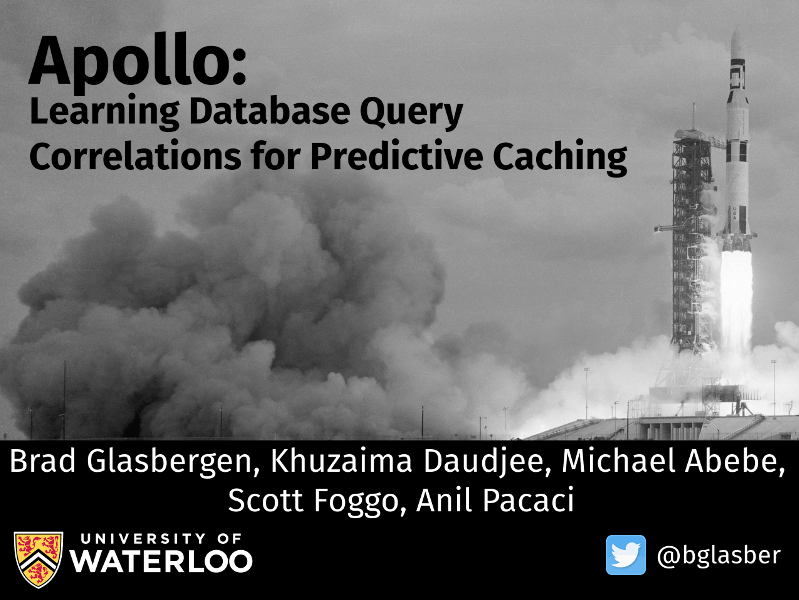
\includegraphics[keepaspectratio=true,width=1.03\paperwidth]{title_slide}
\end{frame}

\begin{frame}{Simple Web Application Architecture}
    \begin{figure}
        \center
        \hspace*{-1cm}
        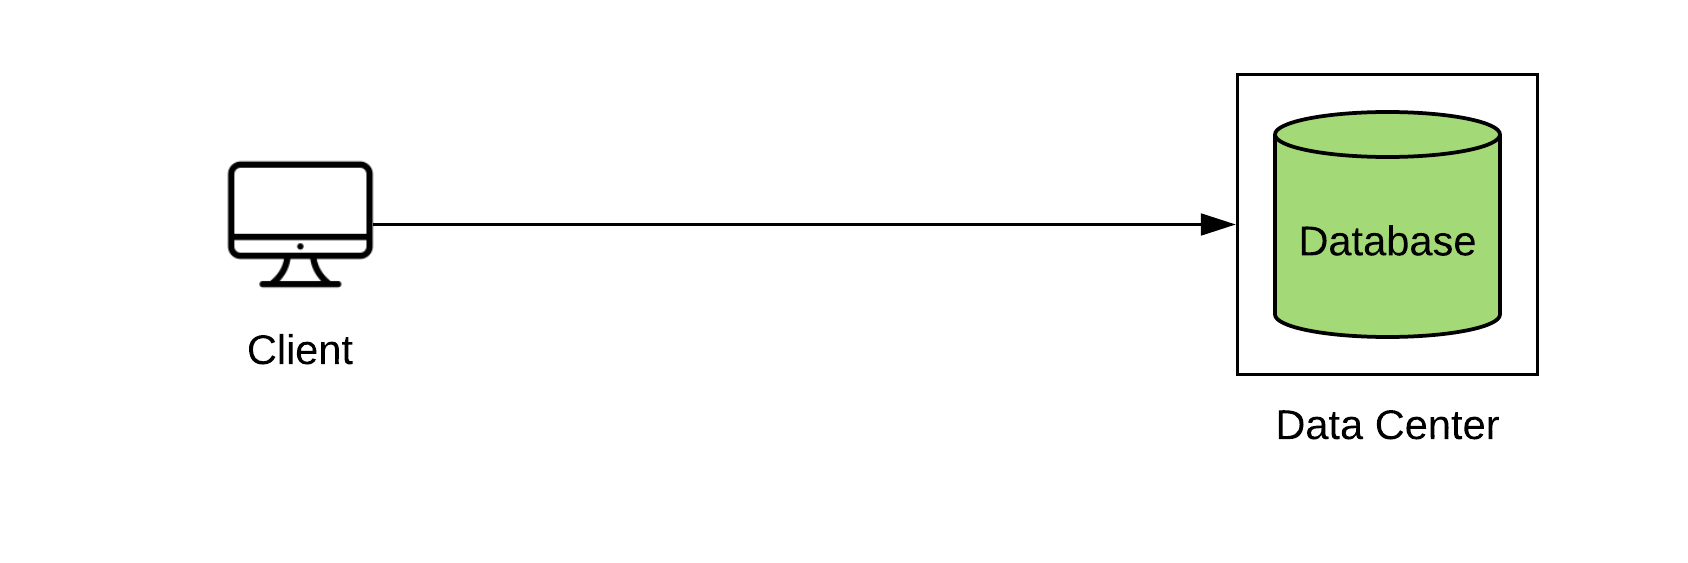
\includegraphics[scale=0.2]{apollo_intro_arch}
    \end{figure}
\end{frame}


\begin{frame}{Worldwide Client/Data Center Distribution}
    \begin{figure}
        \center
        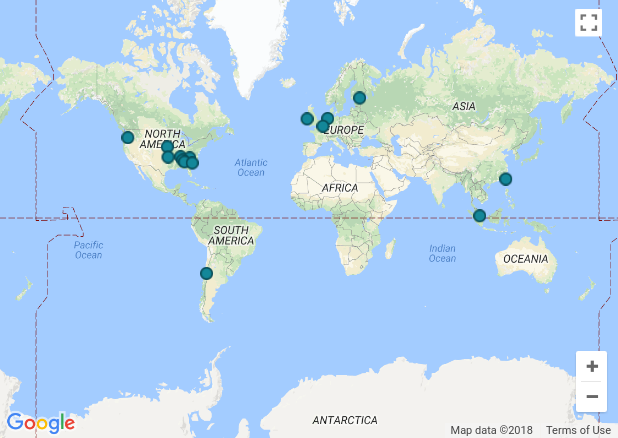
\includegraphics[scale=0.45]{apollo_google_dc}
    \end{figure}
\end{frame}

\begin{frame}{Worldwide Client/Data Center Distribution}
    \begin{figure}
        \center
        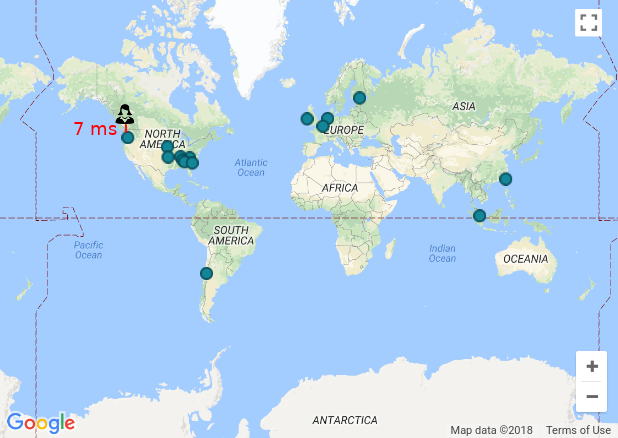
\includegraphics[scale=0.45]{apollo_google_vancouver}
    \end{figure}
\end{frame}

\begin{frame}{Worldwide Client/Data Center Distribution}
    \begin{figure}
        \center
        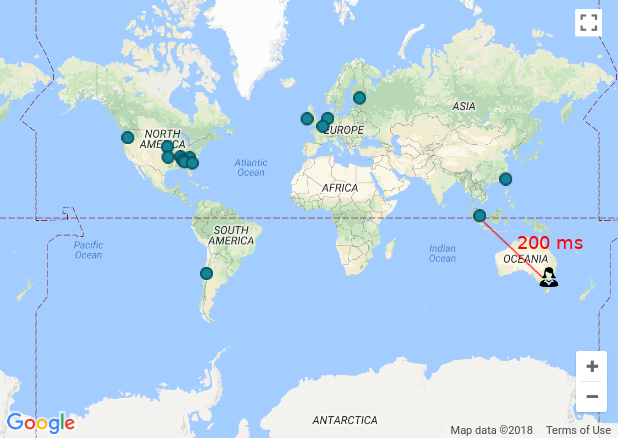
\includegraphics[scale=0.45]{apollo_google_oceania}
    \end{figure}
\end{frame}

\begin{frame}{Latency Effects on Clients}
    Increased latency reduces \alert{user engagement}, and consequently \alert{revenue}! \\
    \vspace{1cm}

    \small{Schurman et al., ``Performance Related Changes and Their User Impact''. \emph{Velocity}, 2009.}
\end{frame}

\begin{frame}{Edge Caching (Content Delivery Networks)}
    \begin{figure}
        \center
        \hspace*{-1.5cm}
        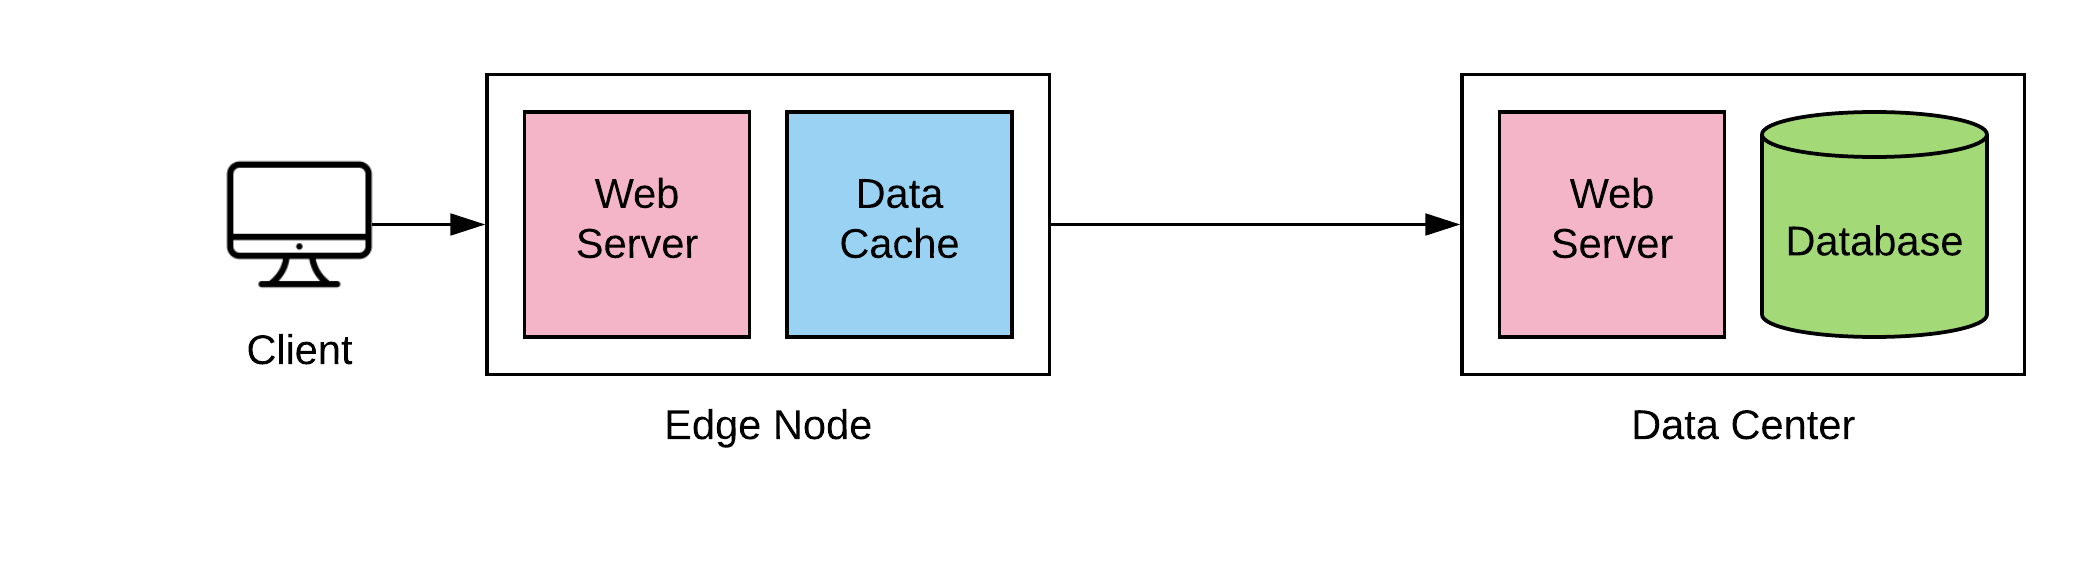
\includegraphics[scale=0.17]{apollo_edge_cache}
    \end{figure}
\end{frame}

\begin{frame}{Worldwide Client/Edge Node Distribution}
    \begin{figure}
        \center
        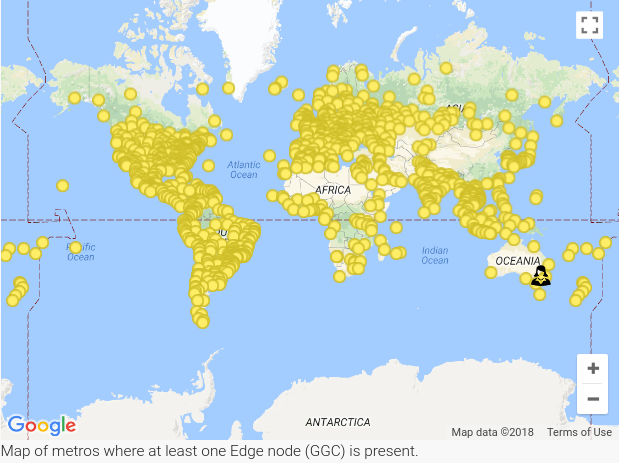
\includegraphics[scale=0.45]{apollo_google_oceania_en}
    \end{figure}
\end{frame}

\begin{frame}{Content Delivery Networks --- A Silver Bullet?}
    \begin{itemize}
        \item{Limited support for non-static data!}
    \end{itemize}
\end{frame}

\begin{comment}
\begin{frame}{Worldwide Client/Edge Node Distribution}
    \begin{figure}
        \center
        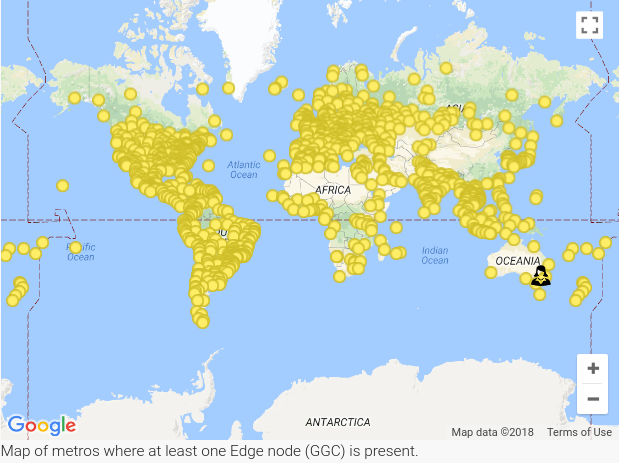
\includegraphics[scale=0.45]{apollo_google_oceania_en}
    \end{figure}
\end{frame}
\end{comment}

\begin{frame}{Static Data Edge Cache Architecture}
    \begin{figure}
        \center
        \hspace*{-1.5cm}
        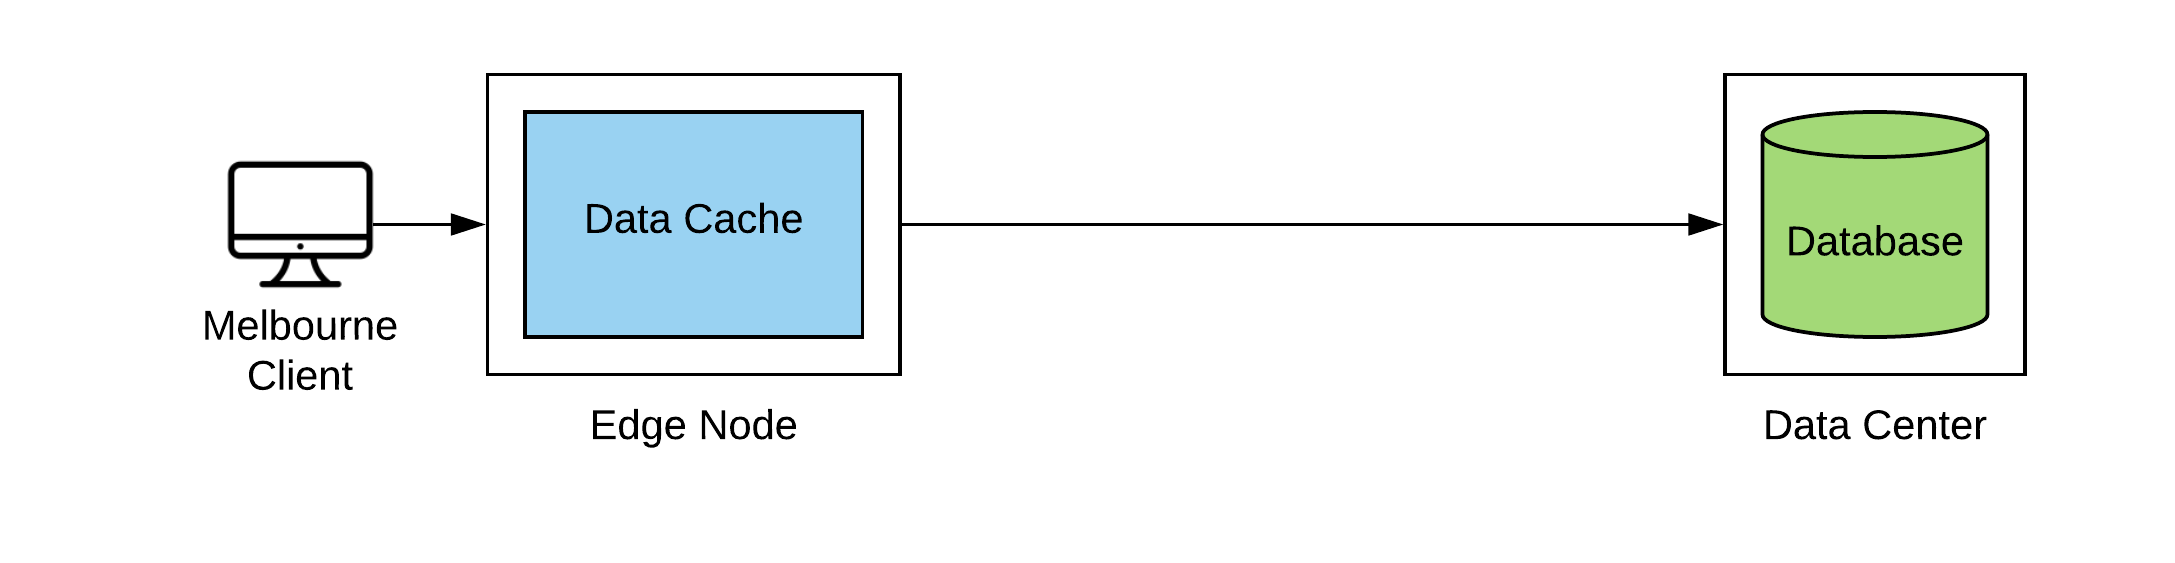
\includegraphics[scale=0.17]{apollo_ec_dbl_0}
    \end{figure}
\end{frame}

\begin{frame}{Extending Edge Cache Support}
    \begin{figure}
        \center
        \hspace*{-1.5cm}
        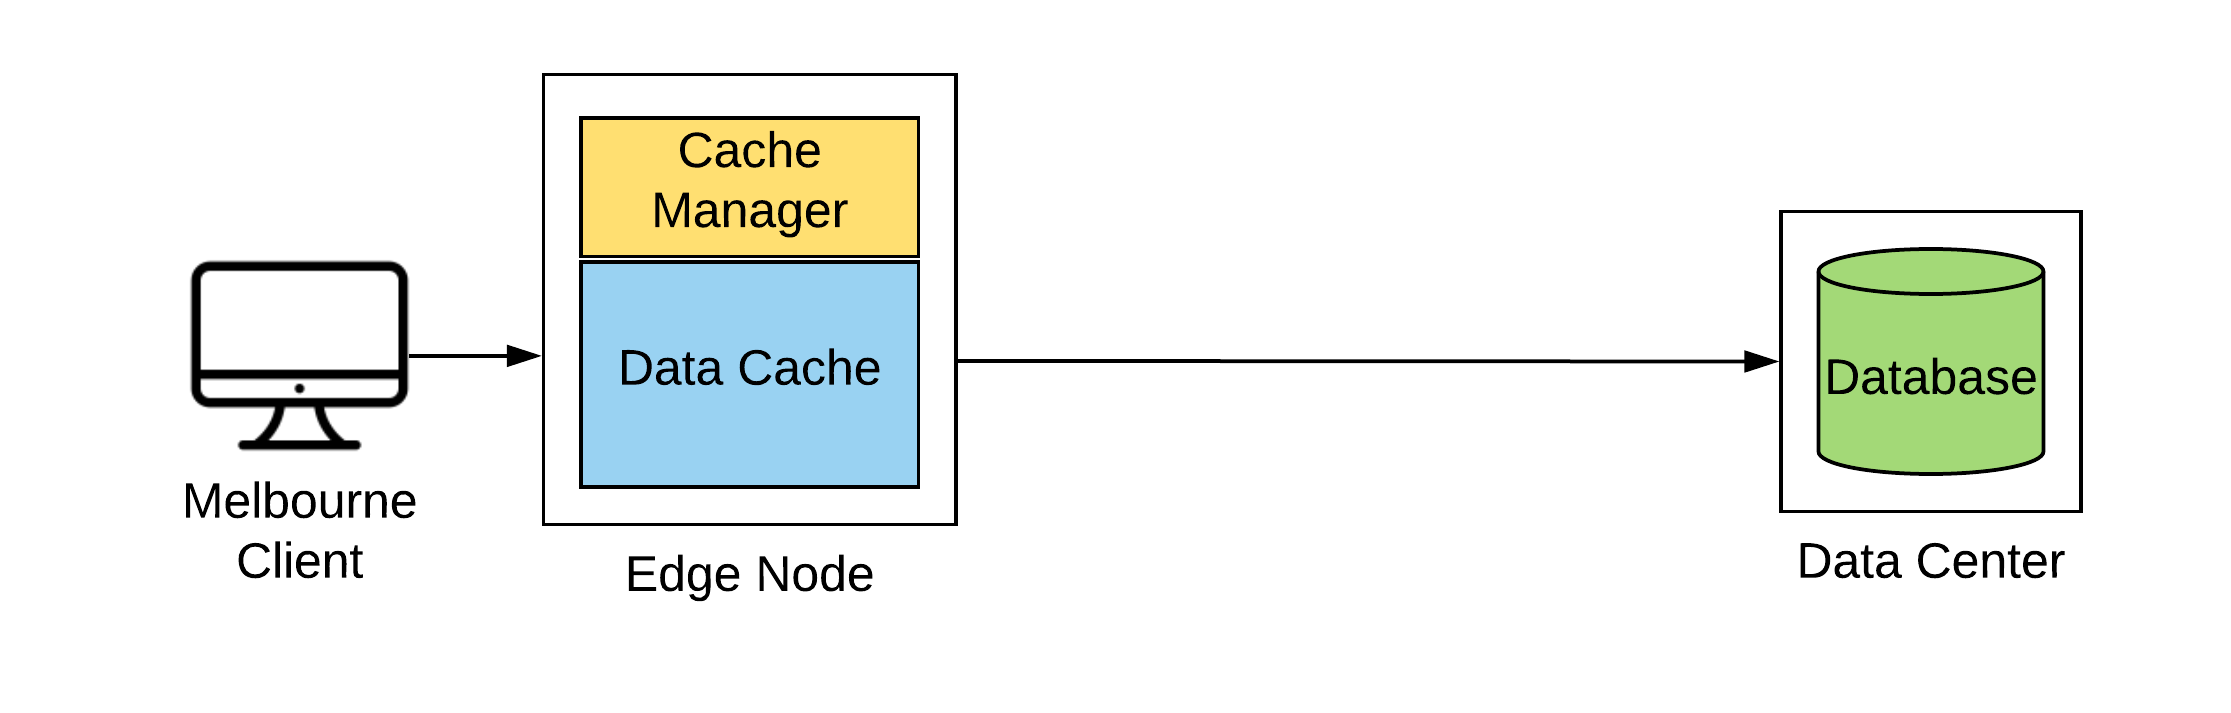
\includegraphics[scale=0.17]{apollo_ec_dbl}
    \end{figure}
\end{frame}

\begin{frame}{Extending Edge Cache Support}
    \begin{figure}
        \center
        \hspace*{-1.5cm}
        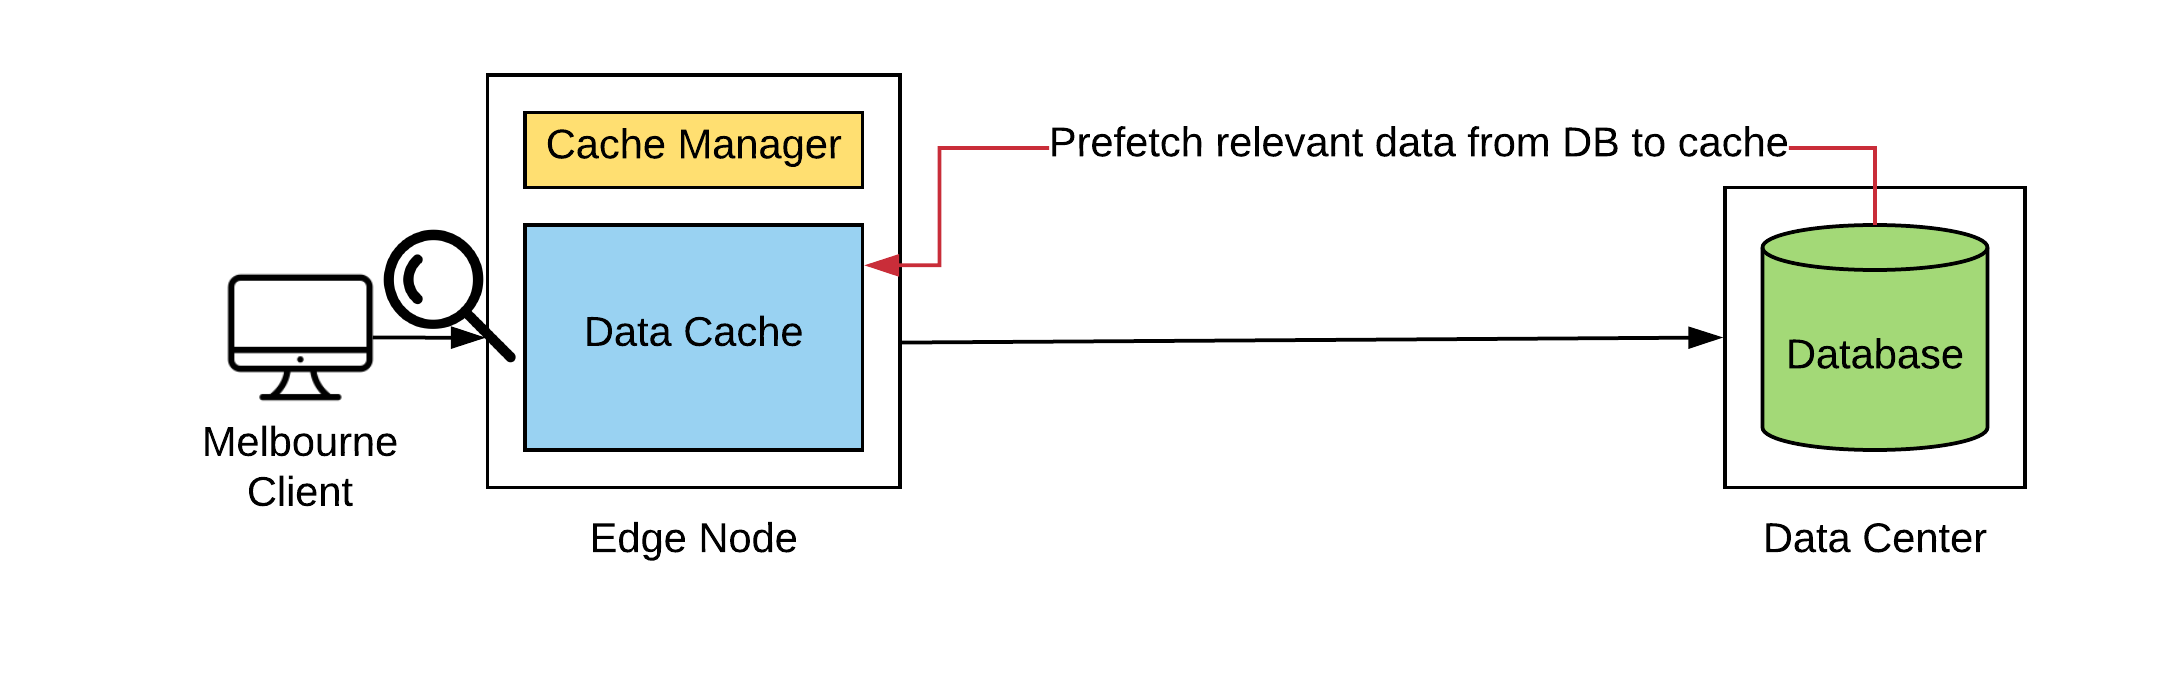
\includegraphics[scale=0.17]{apollo_ec_dbl_learn}
    \end{figure}
\end{frame}

\begin{frame}[fragile]{Dynamic Data Requests (TPC-W Benchmark)}
    \begin{lstlisting}[
                   language=SQL,
                   basicstyle=\ttfamily,
                   commentstyle=\color{gray},
                   escapeinside={(*@}{@*)},
                ]
1. SELECT (*@ \cfbox{red}{C\_ID} @*) FROM CUSTOMER WHERE 
C_UNAME = @C_UN and C_PASSWD = @C_PAS

2. SELECT MAX(O_ID) FROM ORDERS WHERE
O_C_ID = (*@ \cfbox{red}{@C\_ID} @*)
    \end{lstlisting}

\begin{center}
\end{center}
\end{frame}

\begin{frame}{Predictive Caching}
    \begin{figure}
        \center
        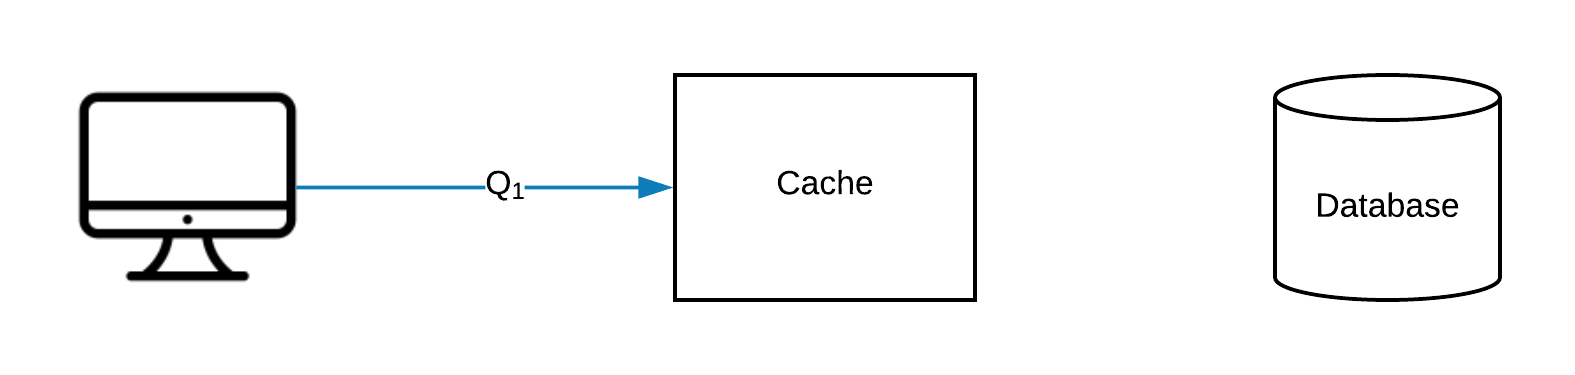
\includegraphics[scale=0.17]{apollo_predictive_execution}
    \end{figure}
\end{frame}

\begin{frame}{Predictive Caching}
    \begin{figure}
        \center
        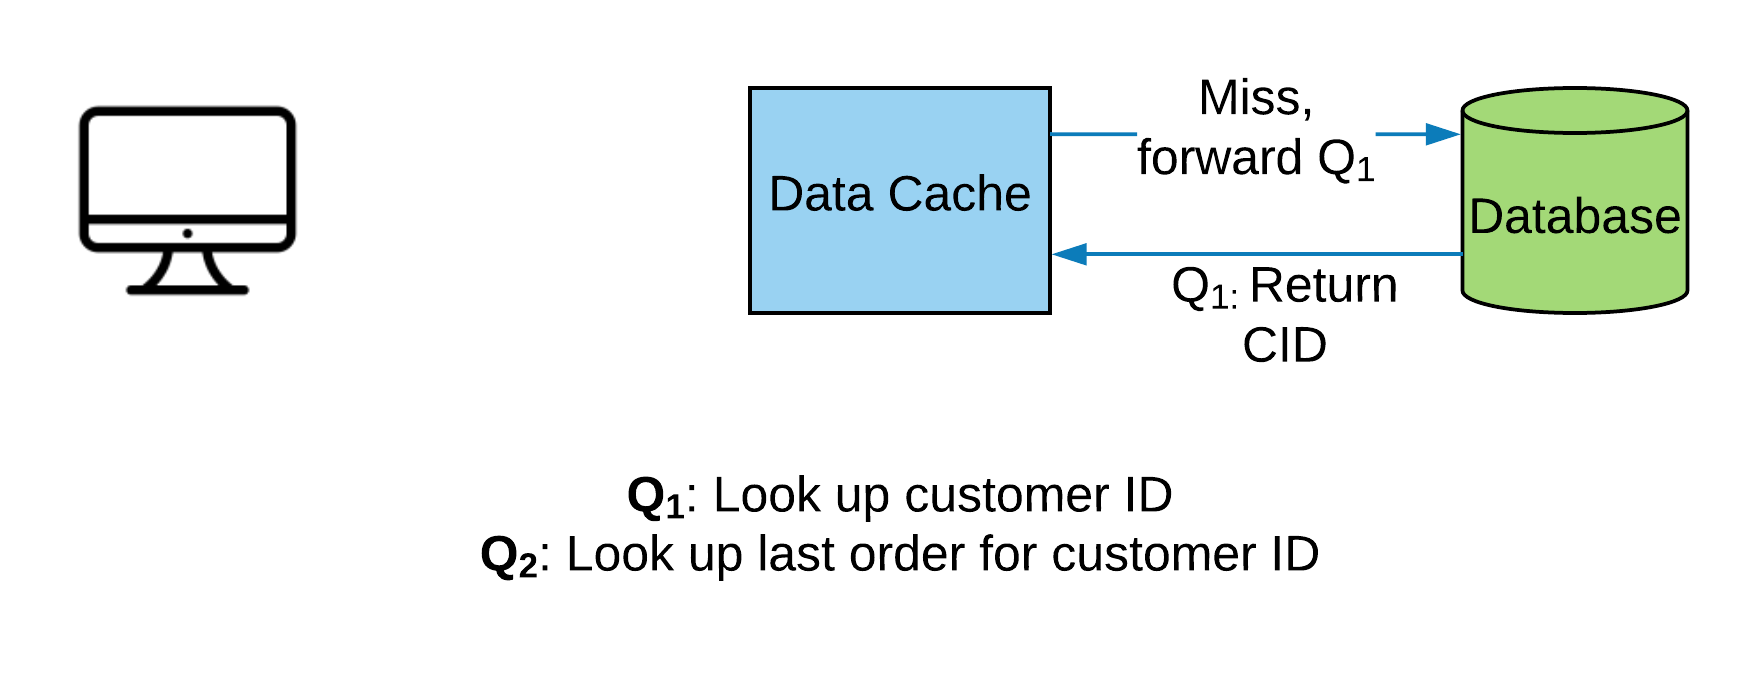
\includegraphics[scale=0.17]{apollo_predictive_execution_2}
    \end{figure}
\end{frame}

\begin{frame}{Predictive Caching}
    \begin{figure}
        \center
        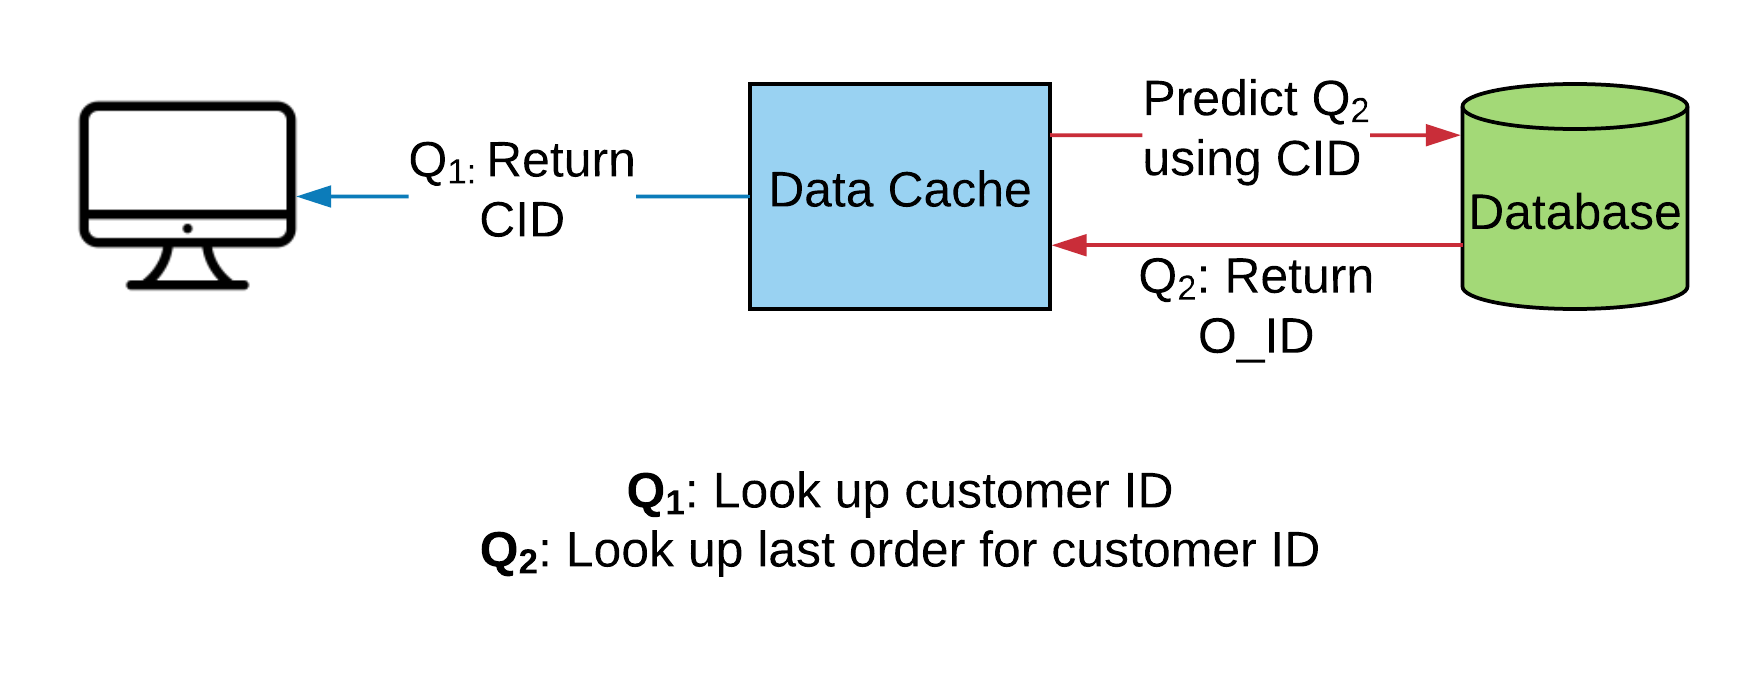
\includegraphics[scale=0.17]{apollo_predictive_execution_4}
    \end{figure}
\end{frame}

\begin{frame}{Predictive Caching}
    \begin{figure}
        \center
        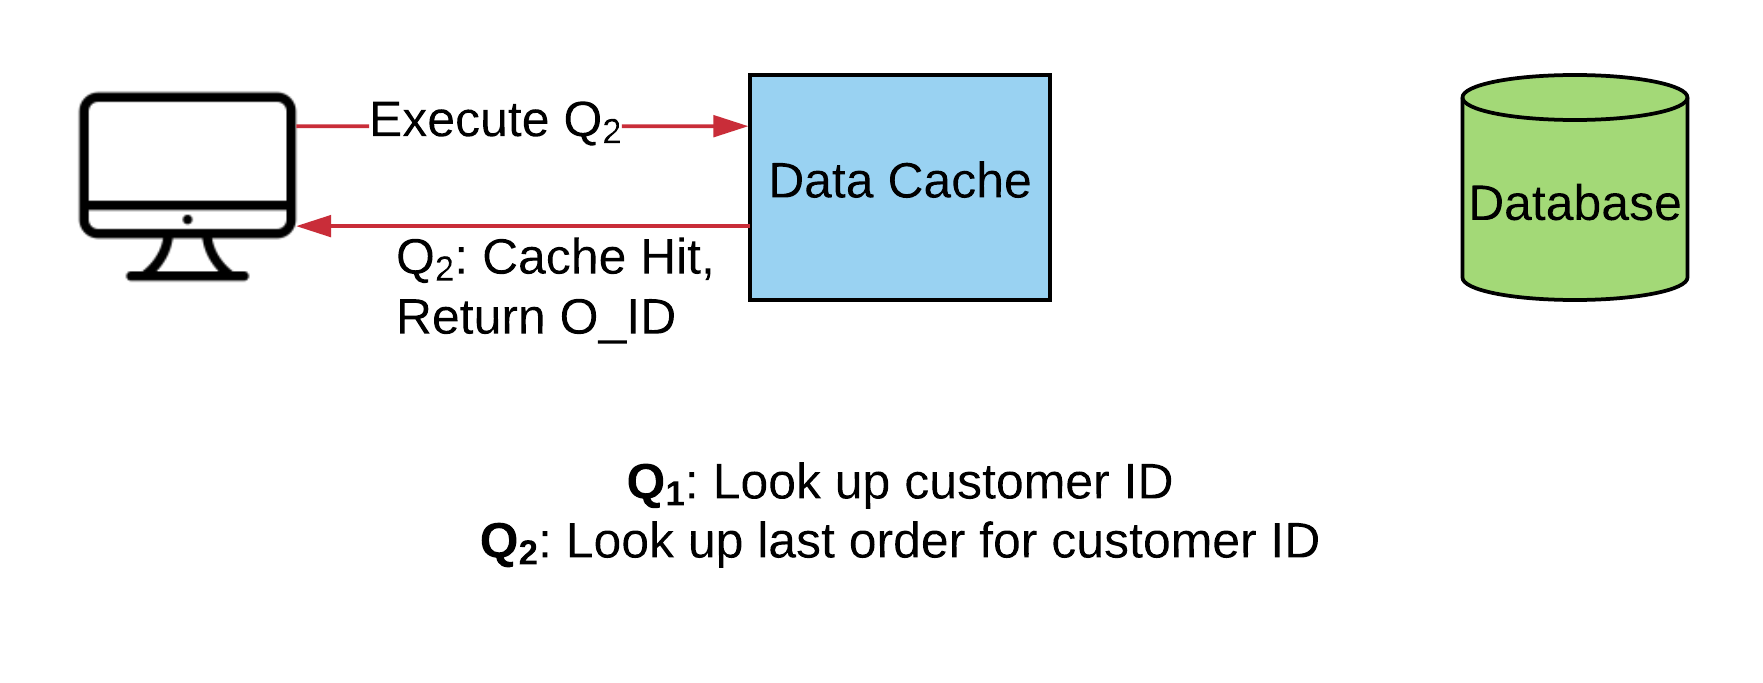
\includegraphics[scale=0.17]{apollo_predictive_execution_5}
    \end{figure}
\end{frame}

\begin{frame}{Apollo: Caching Dynamic Data}
    We developed Apollo, a middleware system that:
    \begin{itemize}
        \visible<2->{
            \item{Uses \alert{online learning} to discover client query patterns.}
        }
        \visible<3->{
            \item{\alert{Predictively executes} and caches query results using these patterns to reduce client response time.}
        }
        \visible<4->{
            \item{Employs a \alert{computationally efficient} means of managing updates to cached data.}
        }
    \end{itemize}
\end{frame}

\begin{frame}{Table of contents}
  \setbeamertemplate{section in toc}[sections numbered]
  \tableofcontents[hideallsubsections]
\end{frame}

\section{Predictive Query Model}


\begin{comment} 
\begin{frame}[fragile]{Apollo Overview}
    \begin{figure}
        \hspace*{-1cm}
        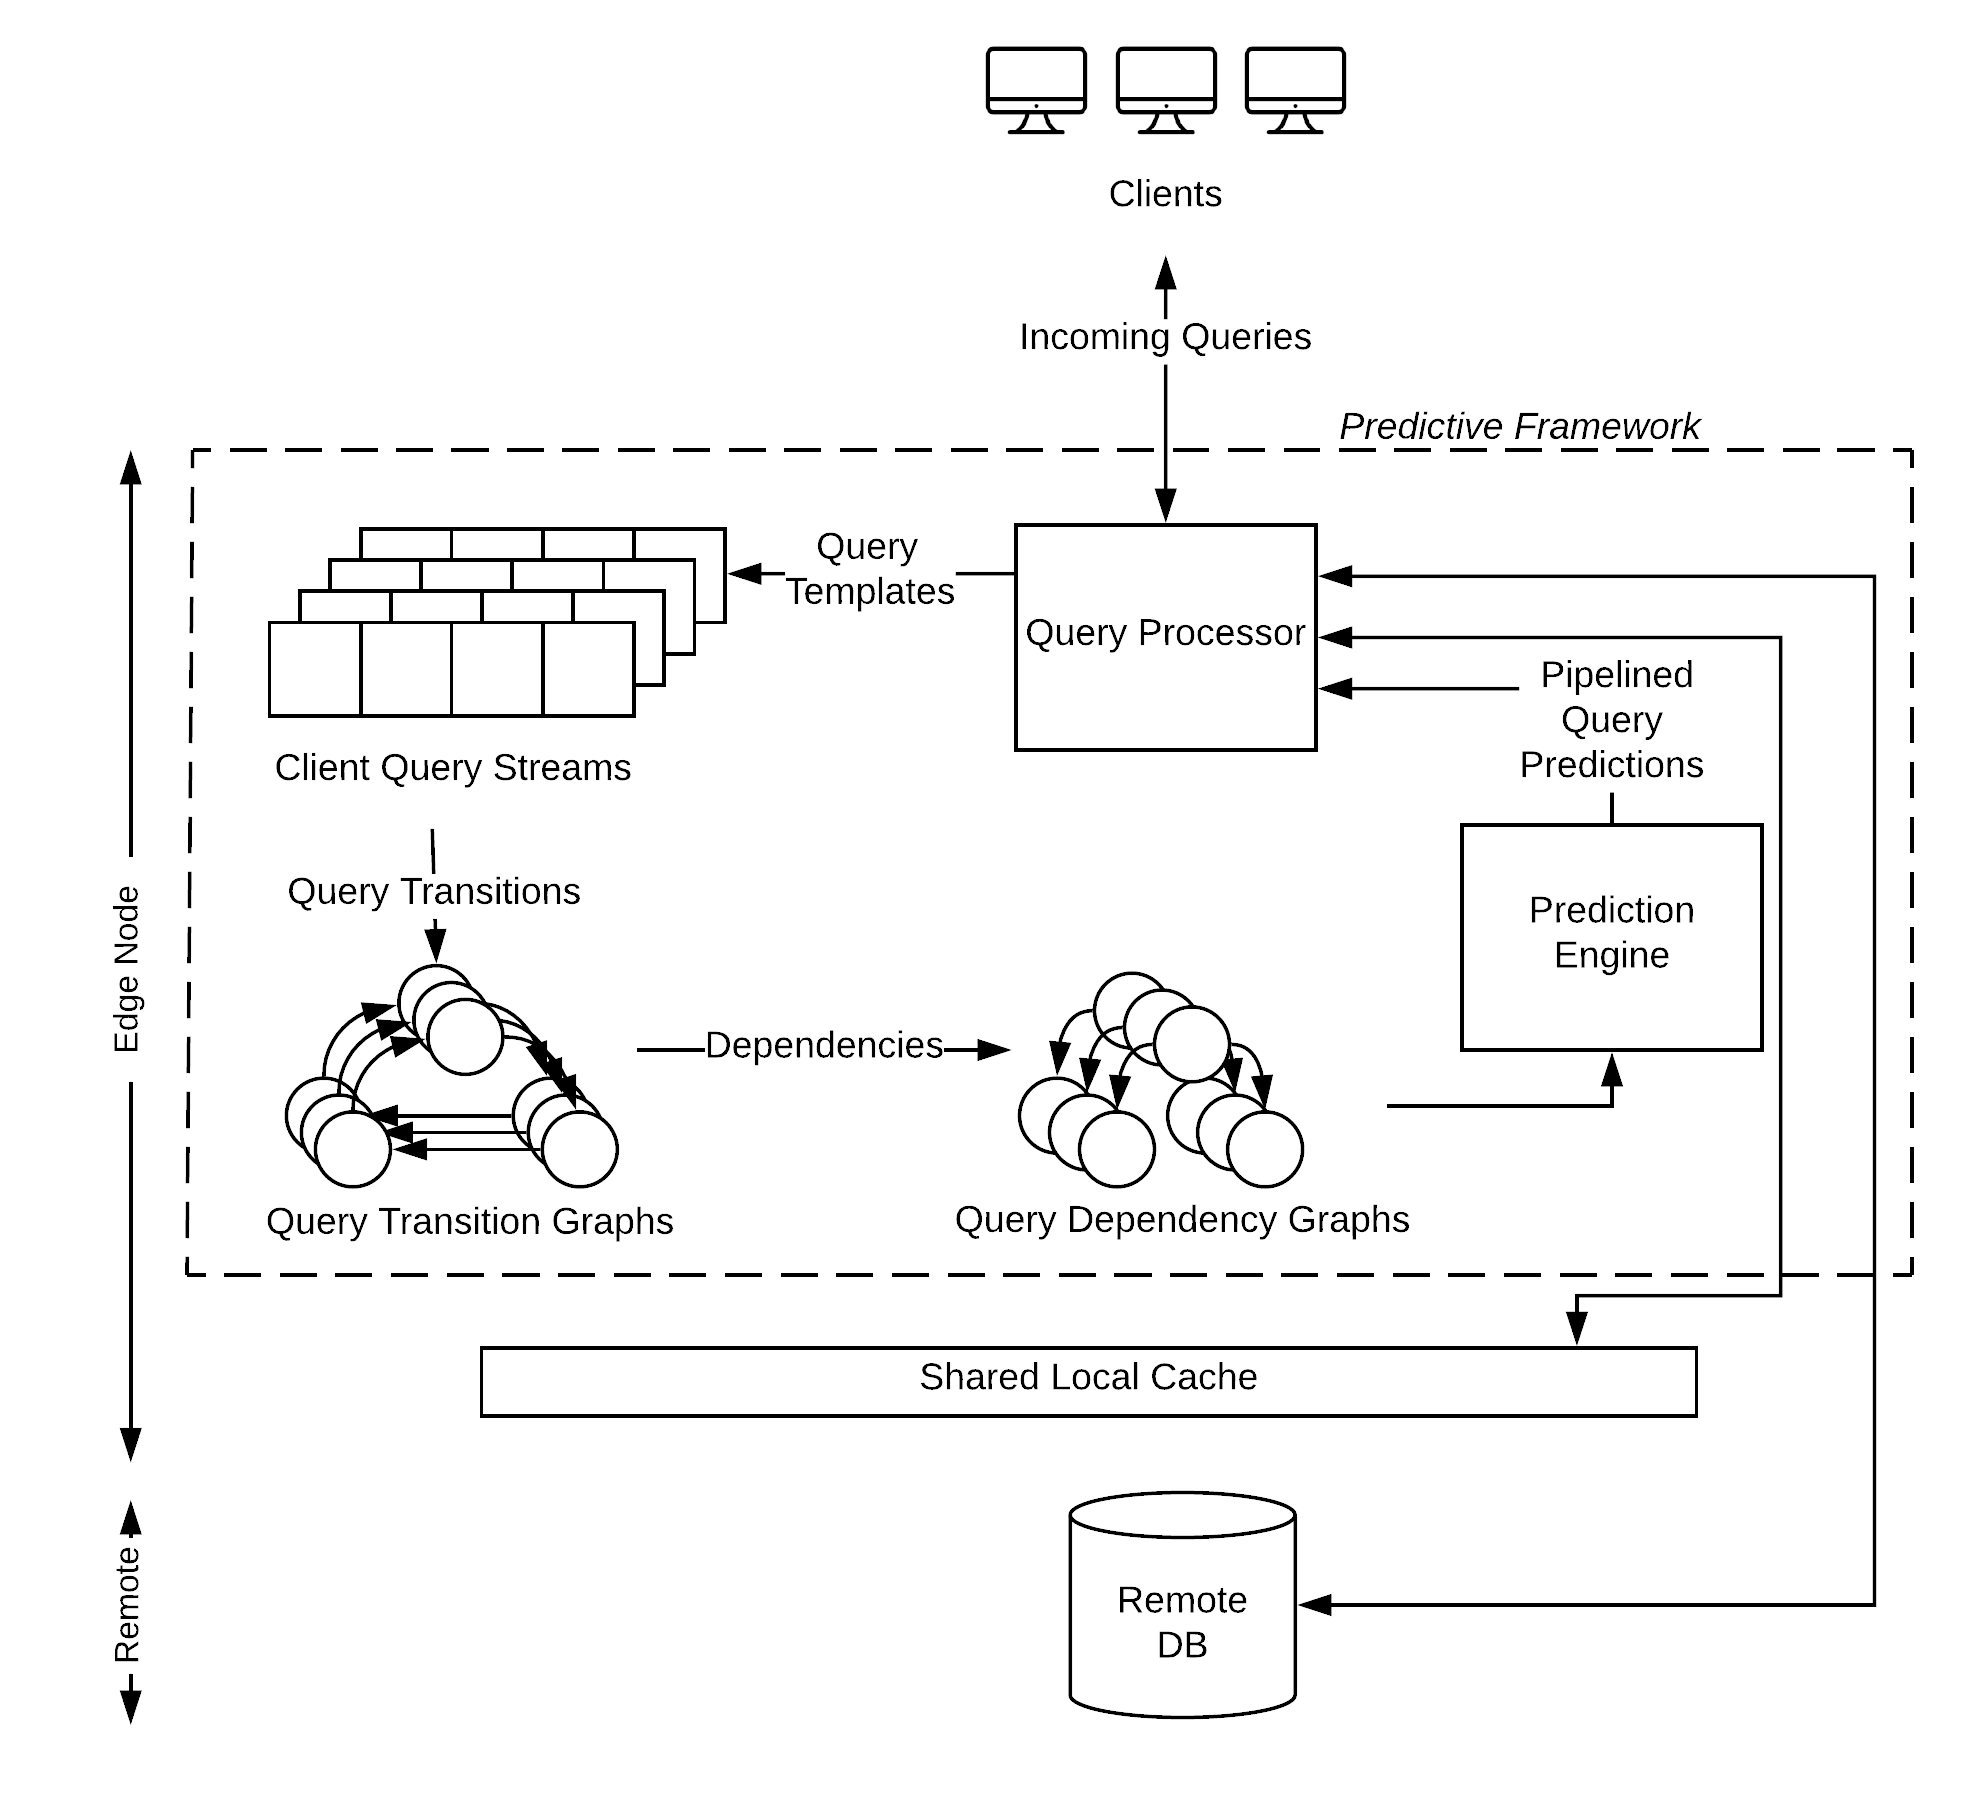
\includegraphics[scale=0.13]{apollo_overview}
    \end{figure}
\end{frame}

\begin{frame}[fragile]{Apollo Overview}
    \begin{figure}
        \hspace*{-1cm}
        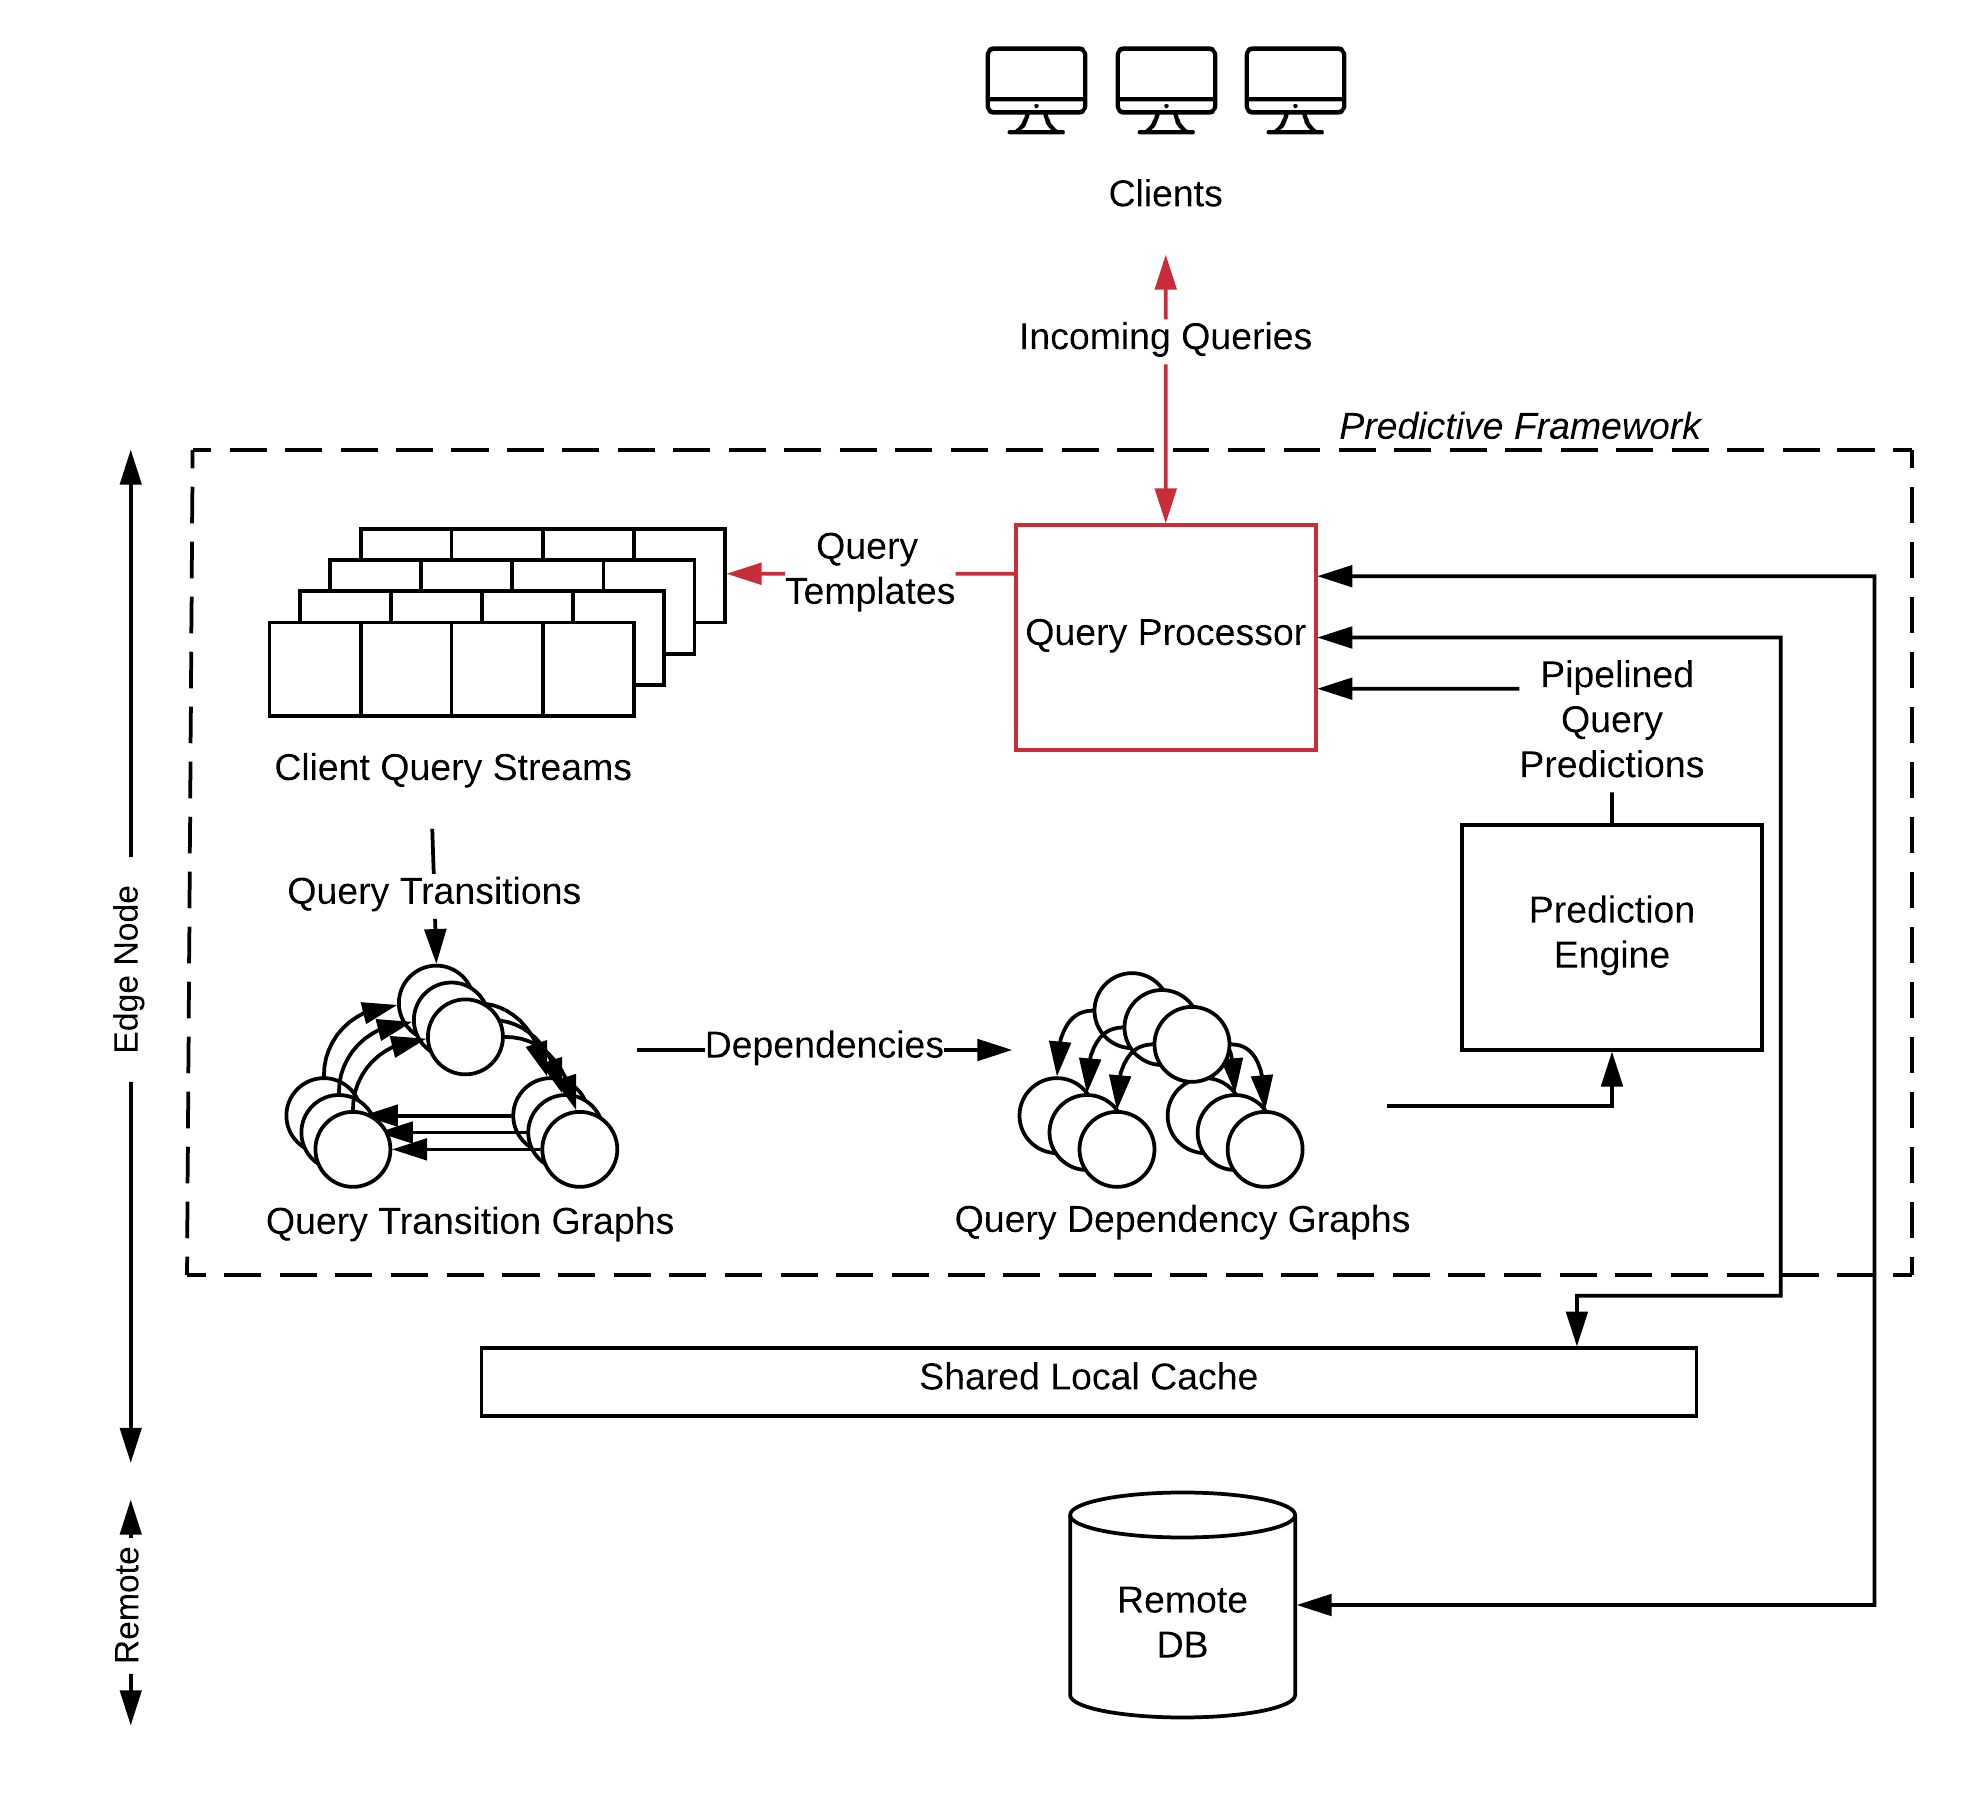
\includegraphics[scale=0.13]{apollo_overview_2}
    \end{figure}
\end{frame}

\begin{frame}[fragile]{Apollo Overview}
    \begin{figure}
        \hspace*{-1cm}
        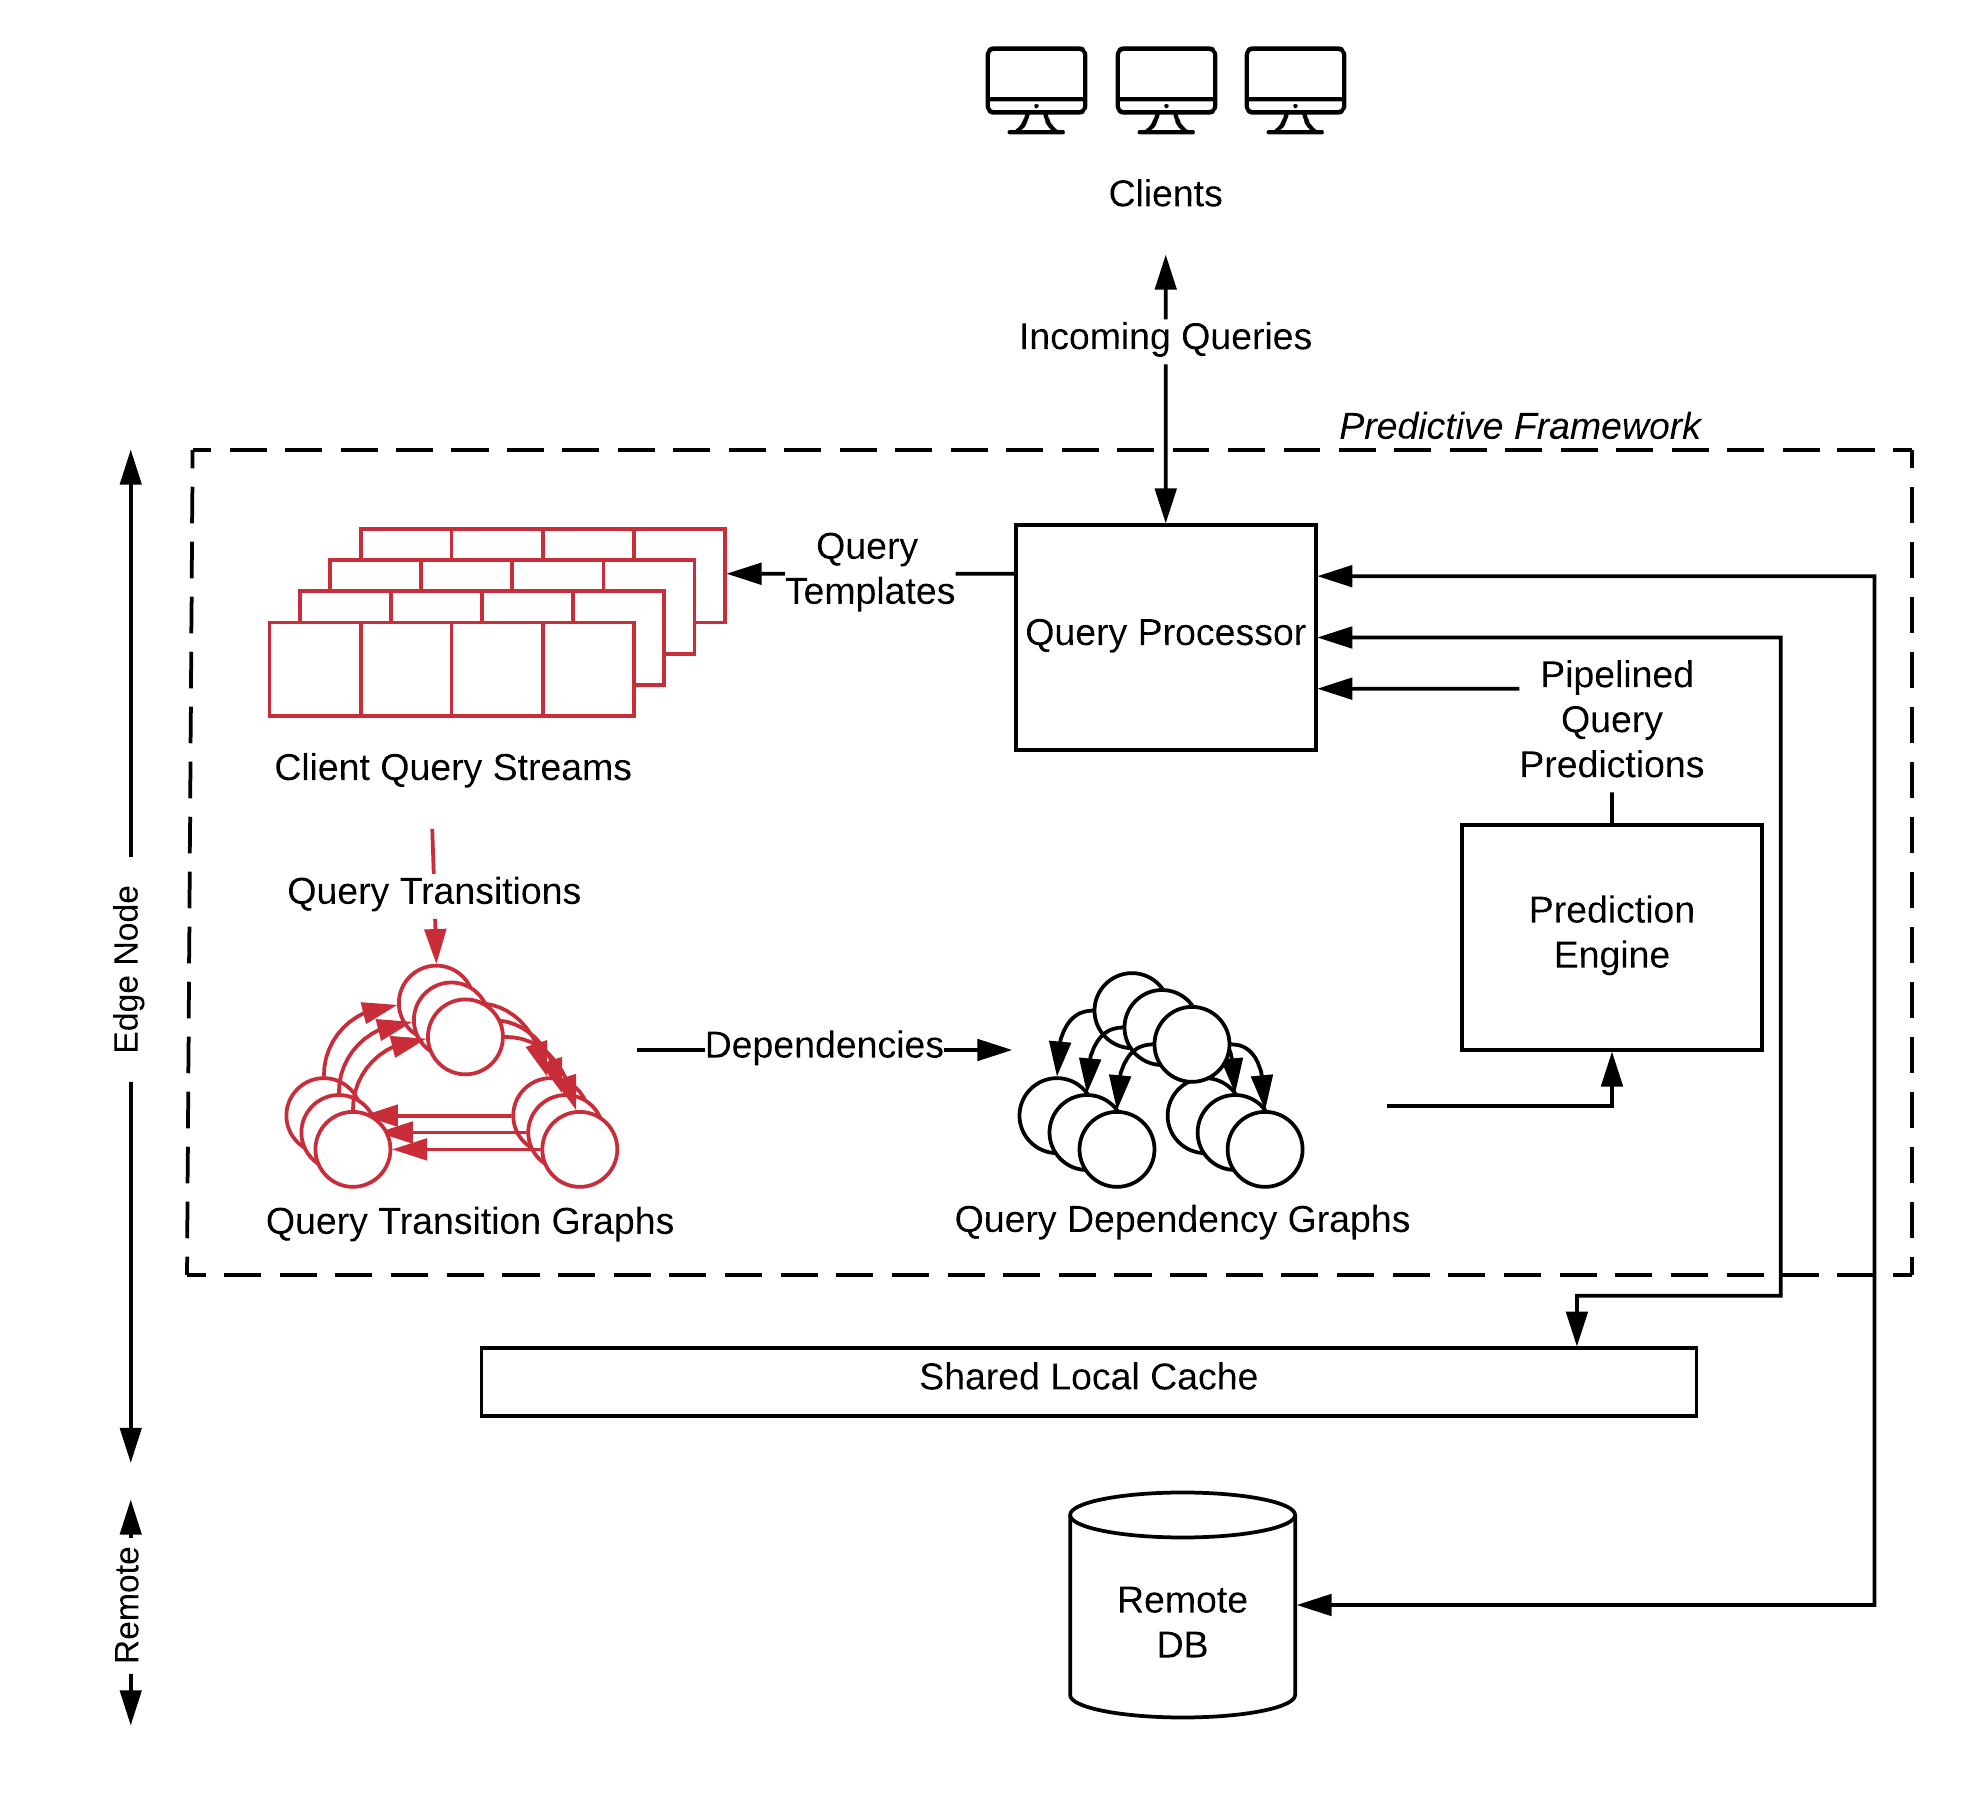
\includegraphics[scale=0.13]{apollo_overview_3}
    \end{figure}
\end{frame}

\begin{frame}[fragile]{Apollo Overview}
    \begin{figure}
        \hspace*{-1cm}
        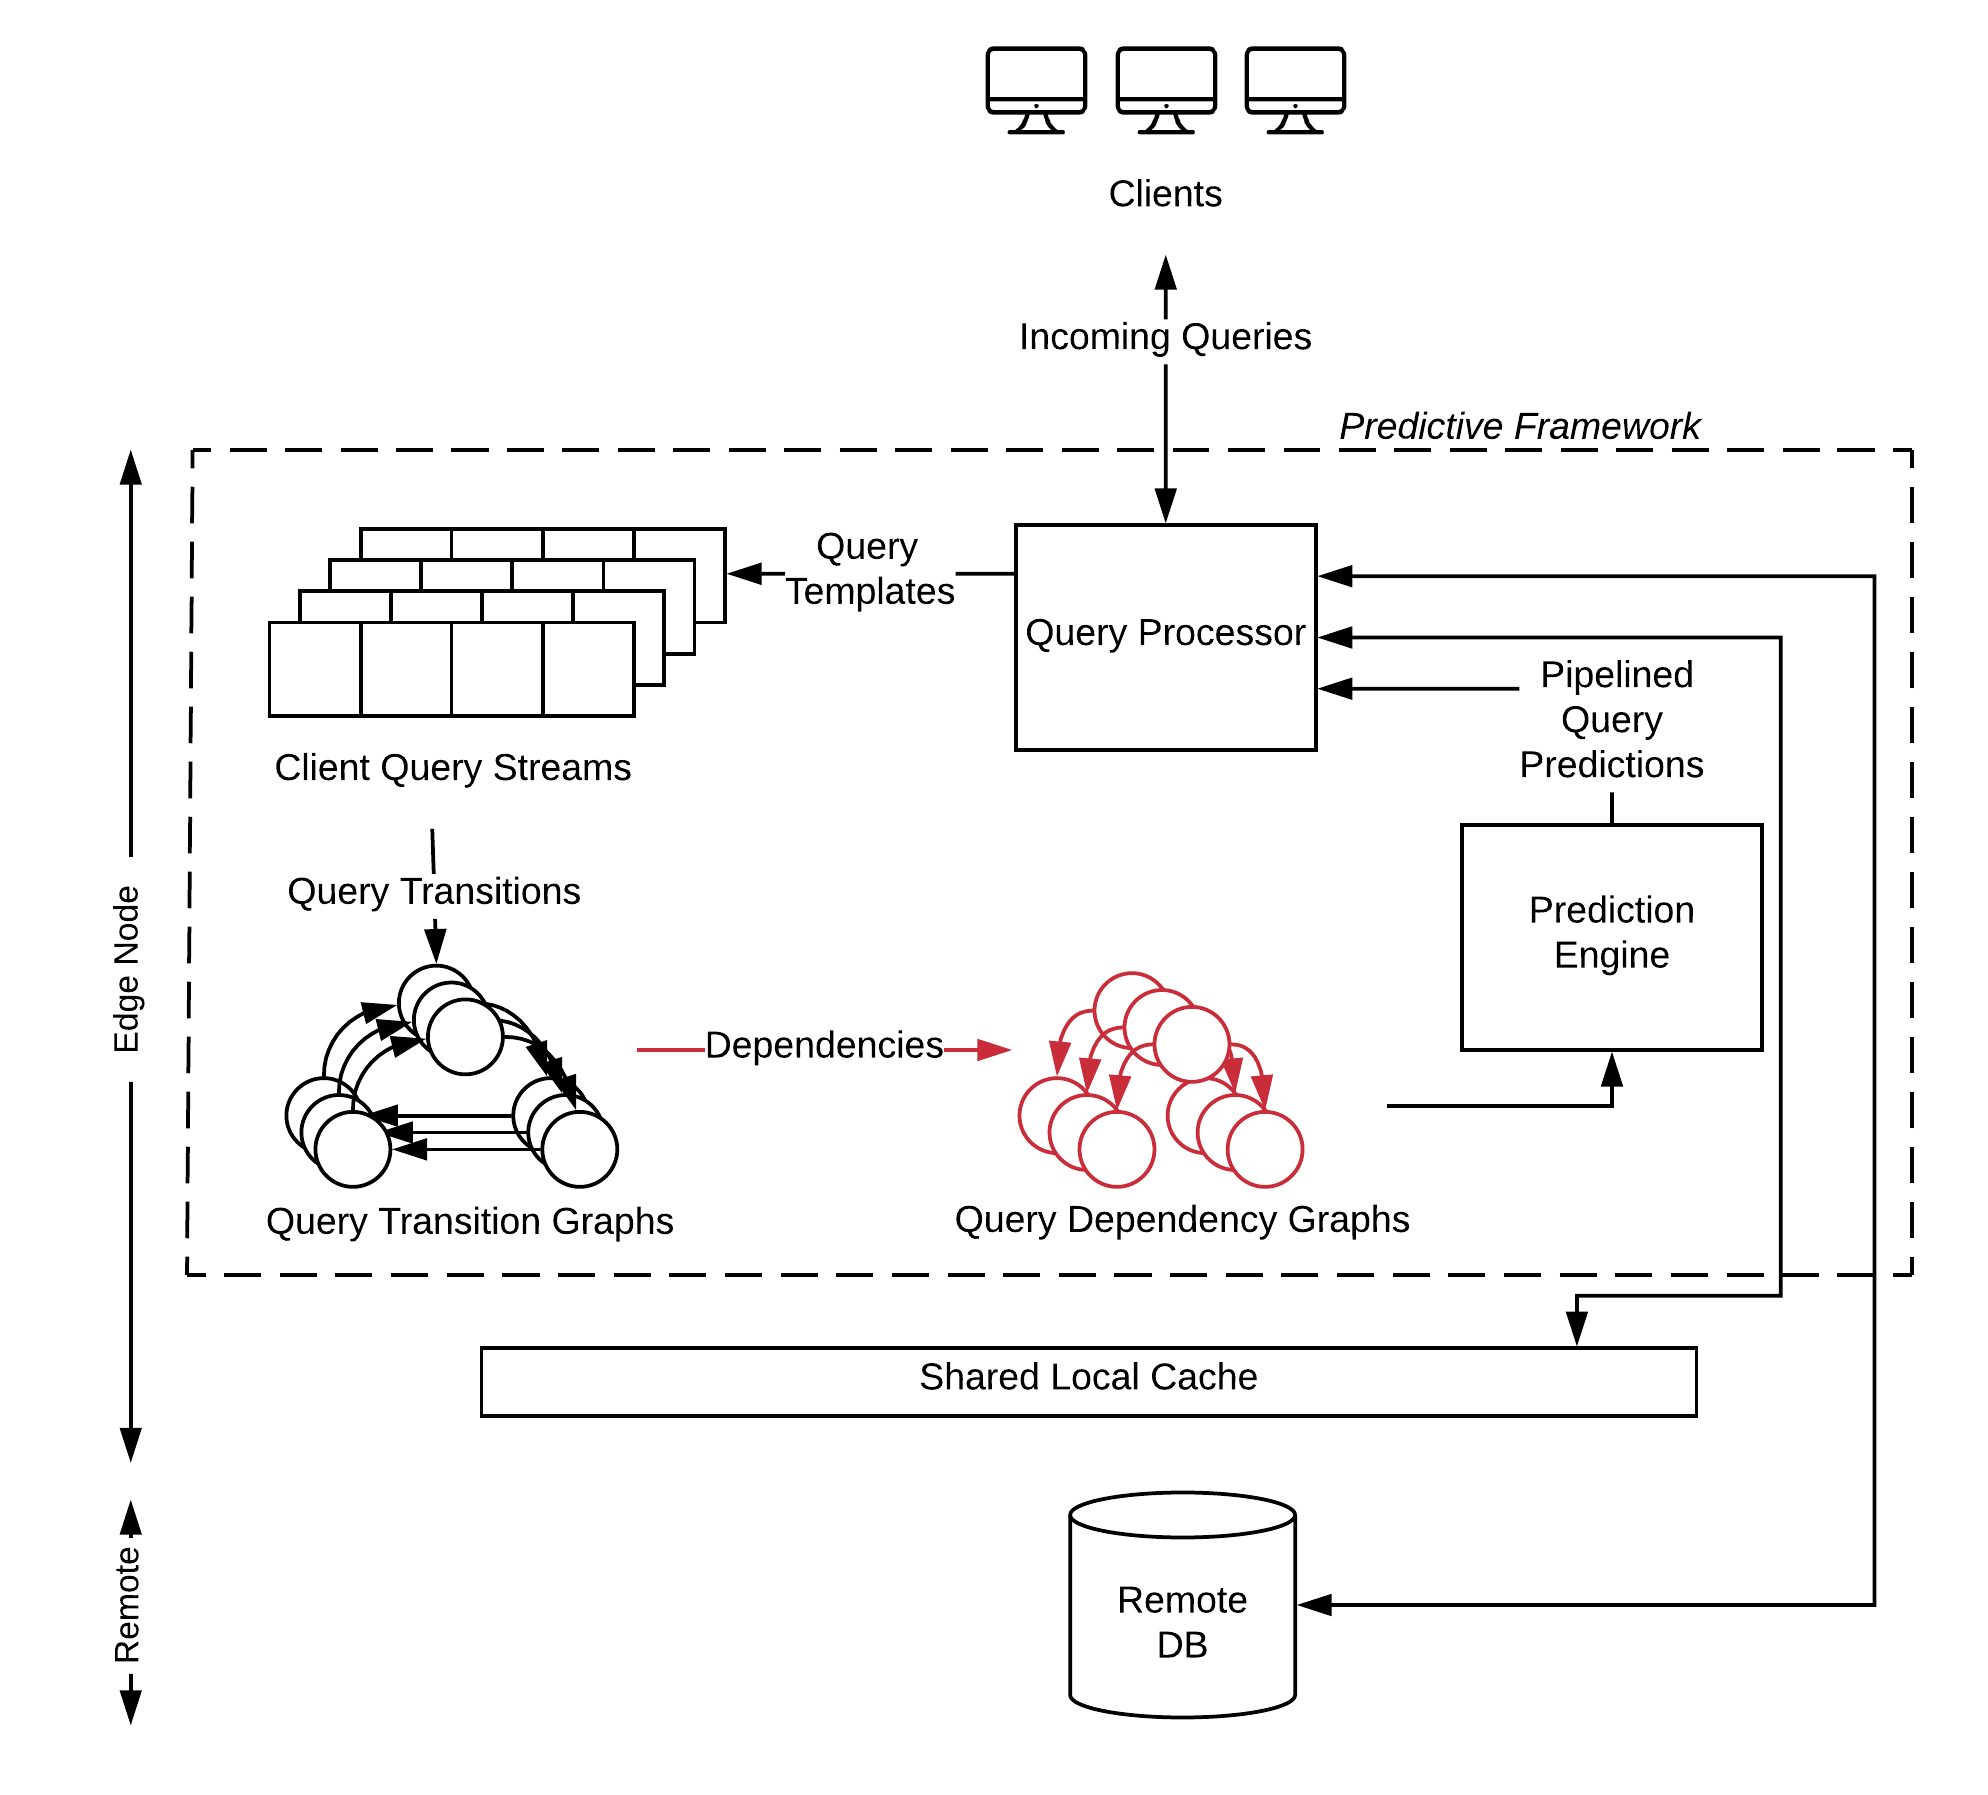
\includegraphics[scale=0.13]{apollo_overview_4}
    \end{figure}
\end{frame}

\begin{frame}[fragile]{Apollo Overview}
    \begin{figure}
        \hspace*{-1cm}
        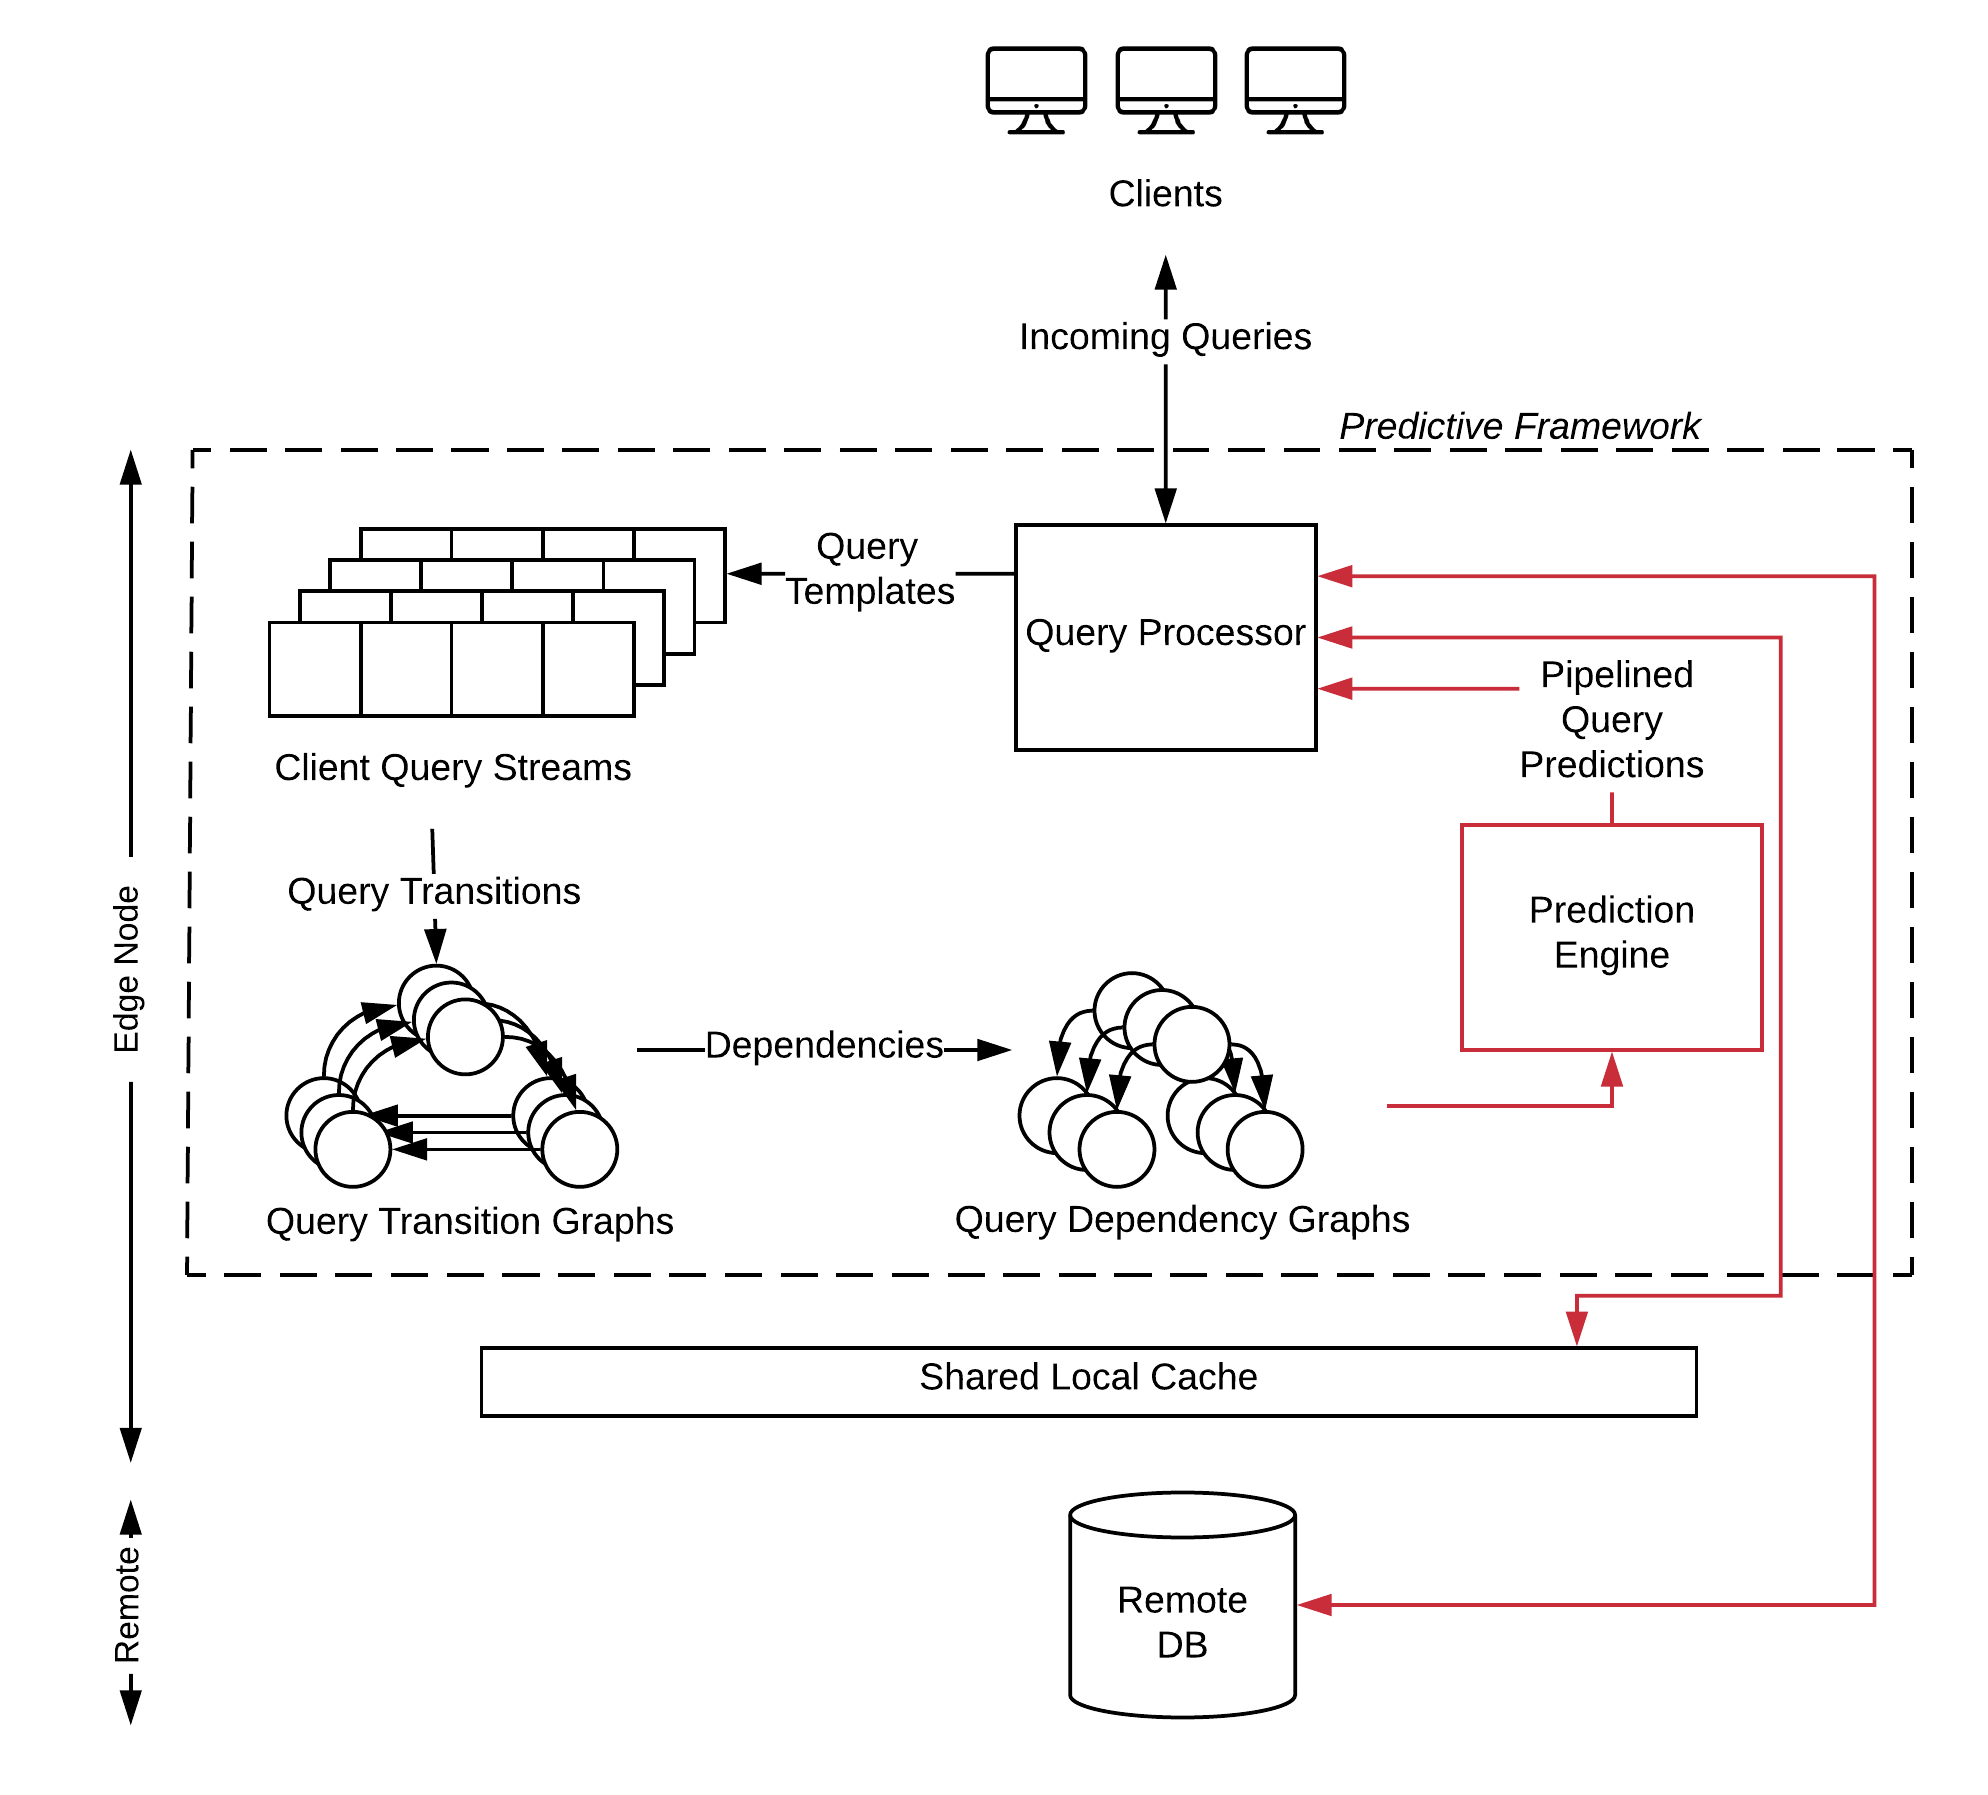
\includegraphics[scale=0.13]{apollo_overview_5}
    \end{figure}
\end{frame}

\begin{frame}[fragile]{Apollo Overview}
    \begin{figure}
        \hspace*{-1cm}
        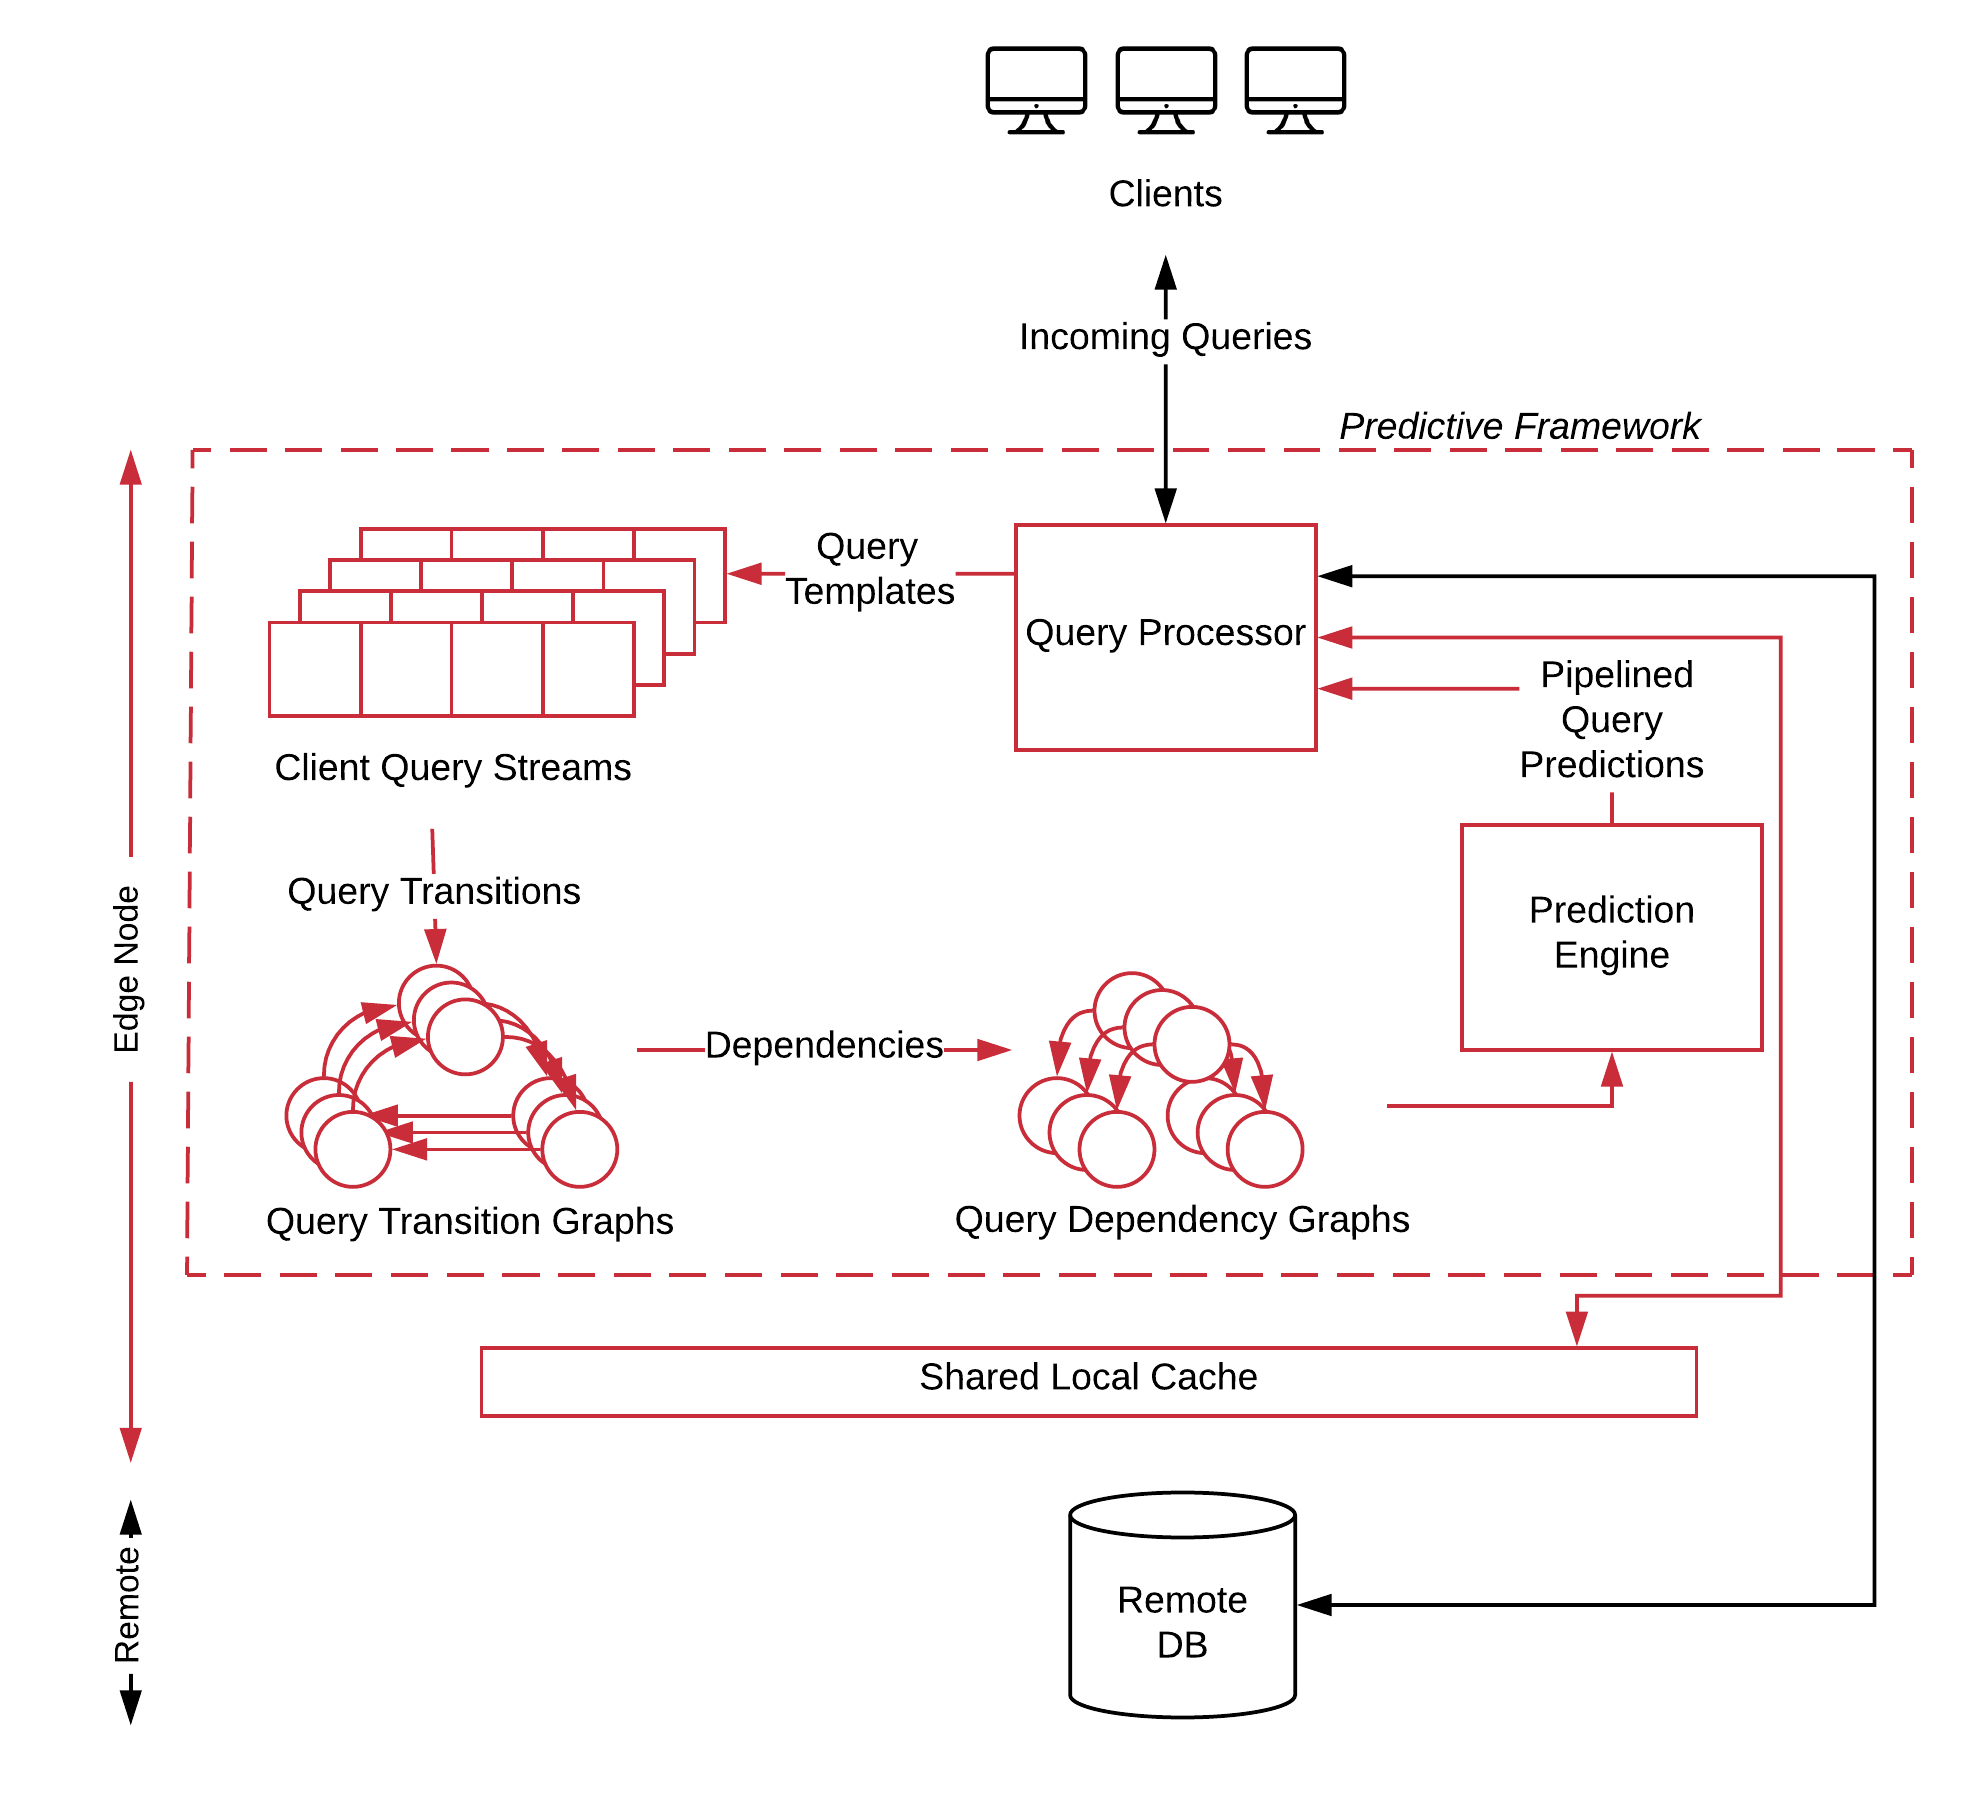
\includegraphics[scale=0.13]{apollo_overview_6}
    \end{figure}
\end{frame}

\begin{frame}[fragile]{Apollo Overview}
    \begin{figure}
        \hspace*{-1cm}
        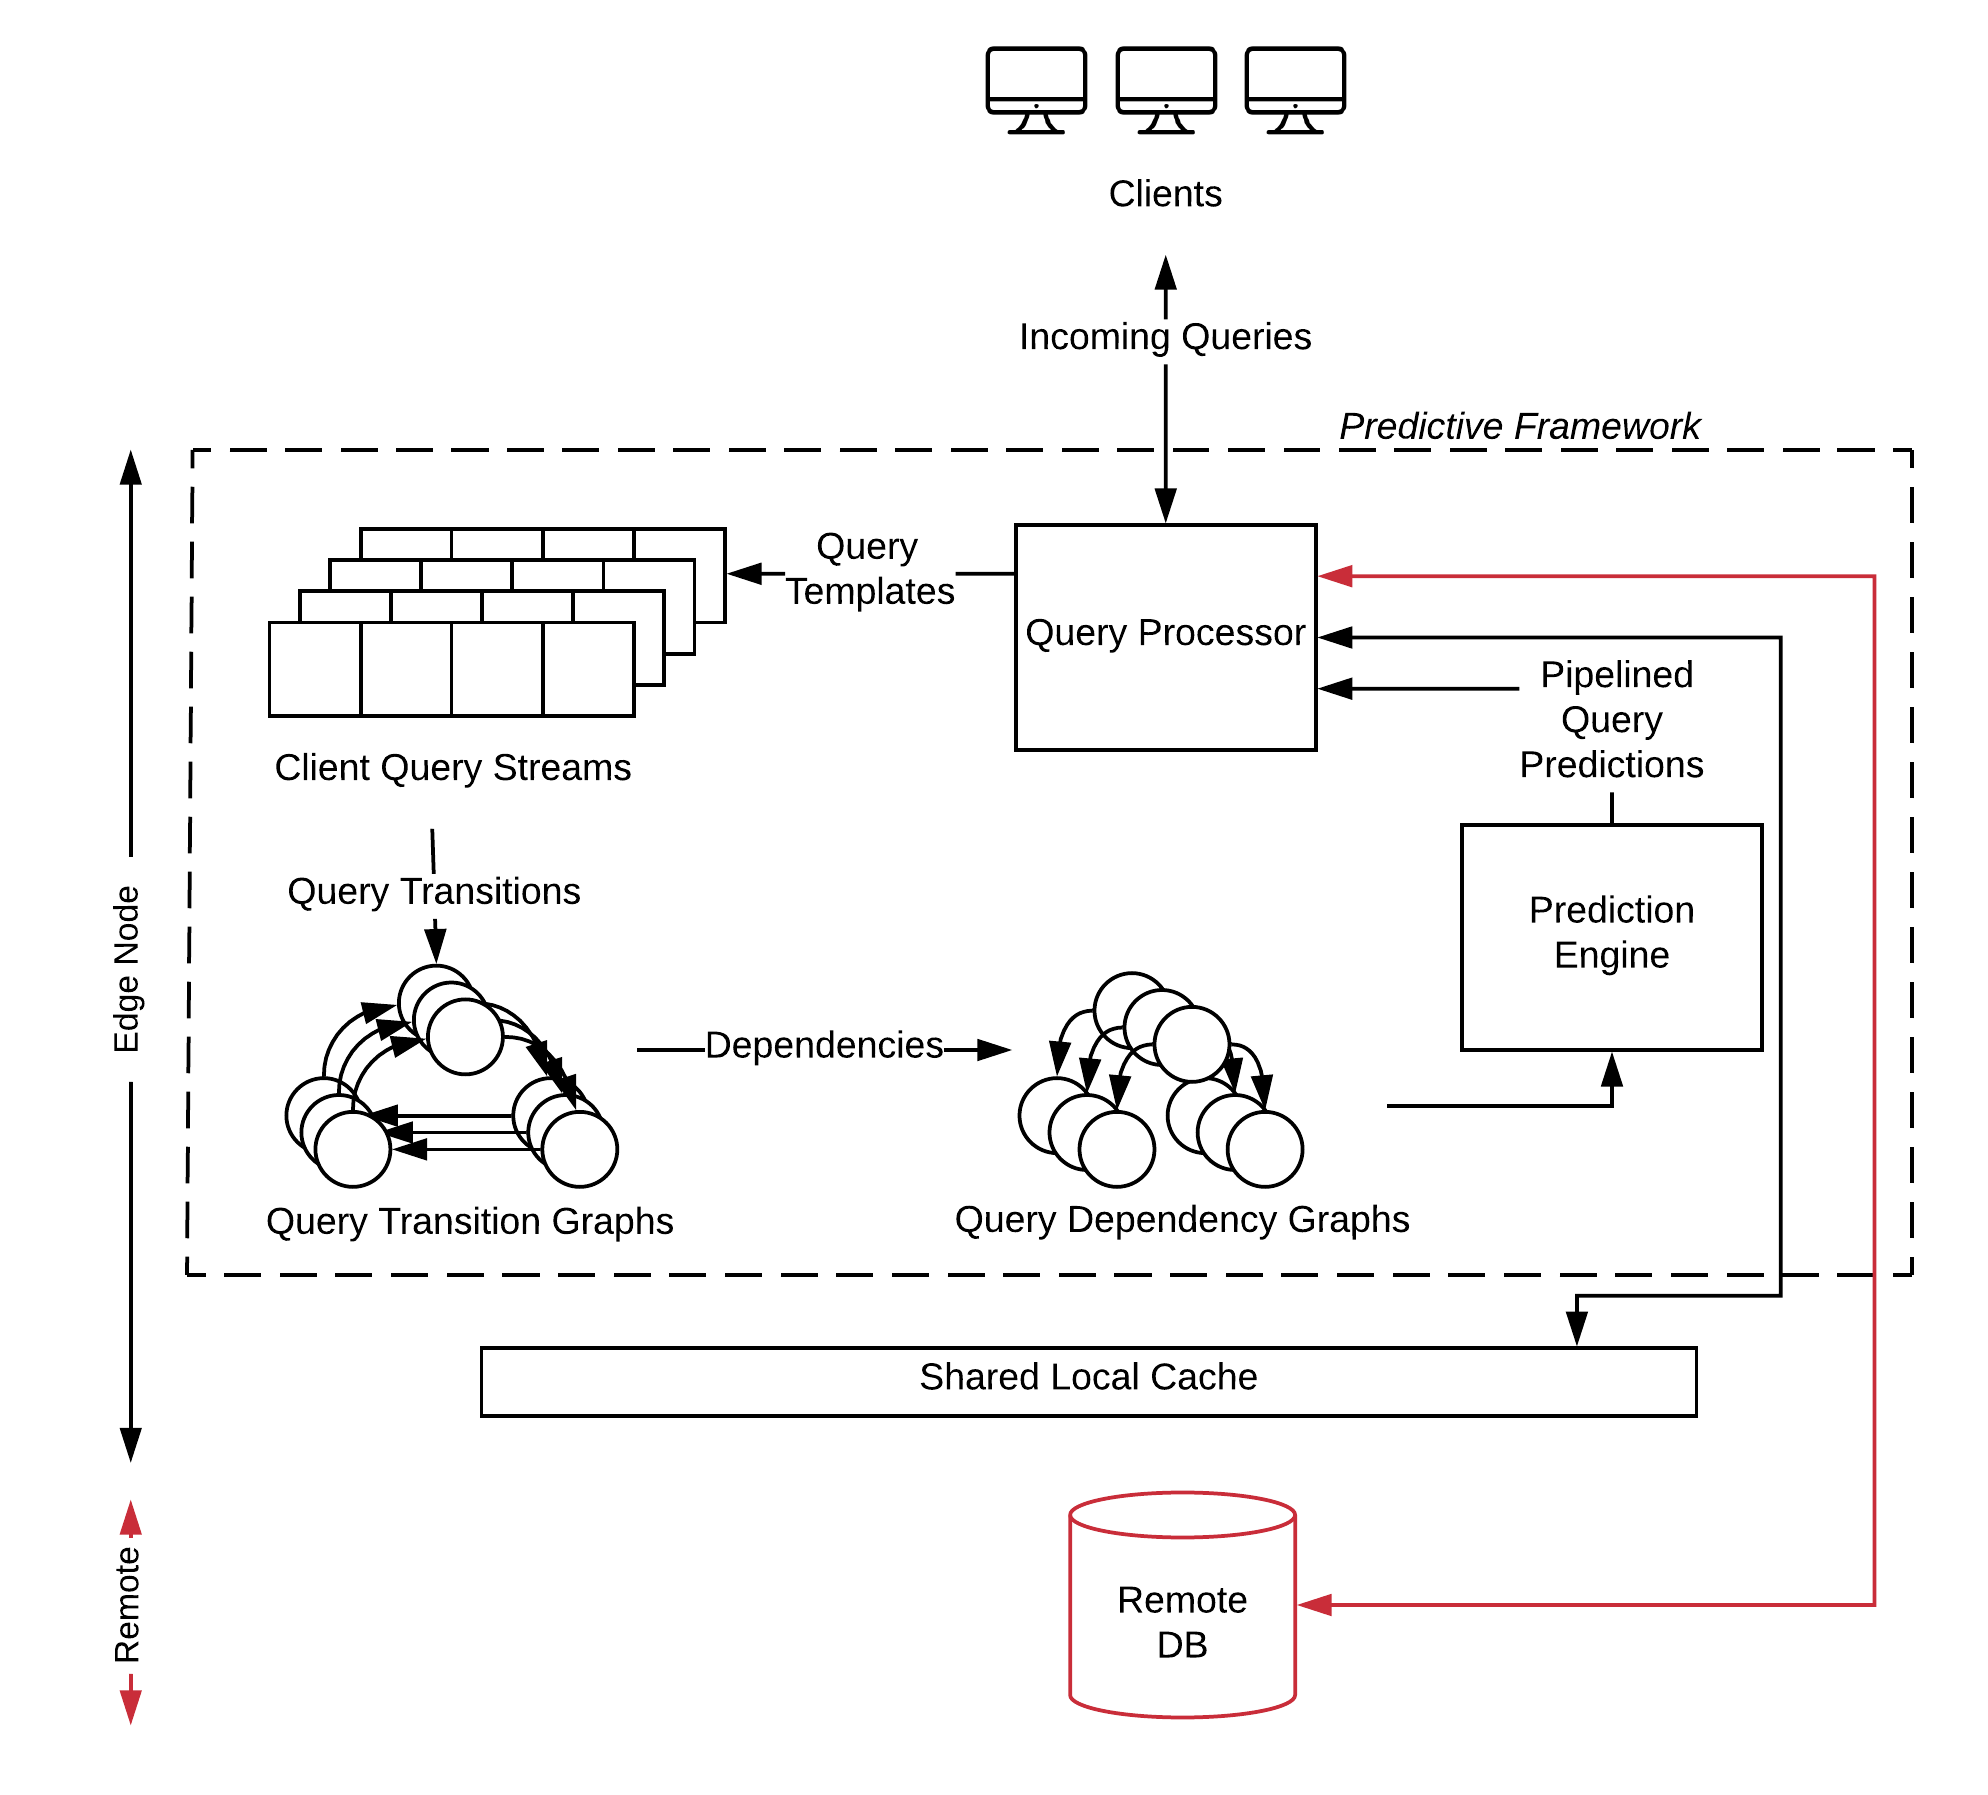
\includegraphics[scale=0.13]{apollo_overview_7}
    \end{figure}
\end{frame}

\end{comment}

\begin{frame}[fragile]{Apollo Overview}
    \begin{figure}
        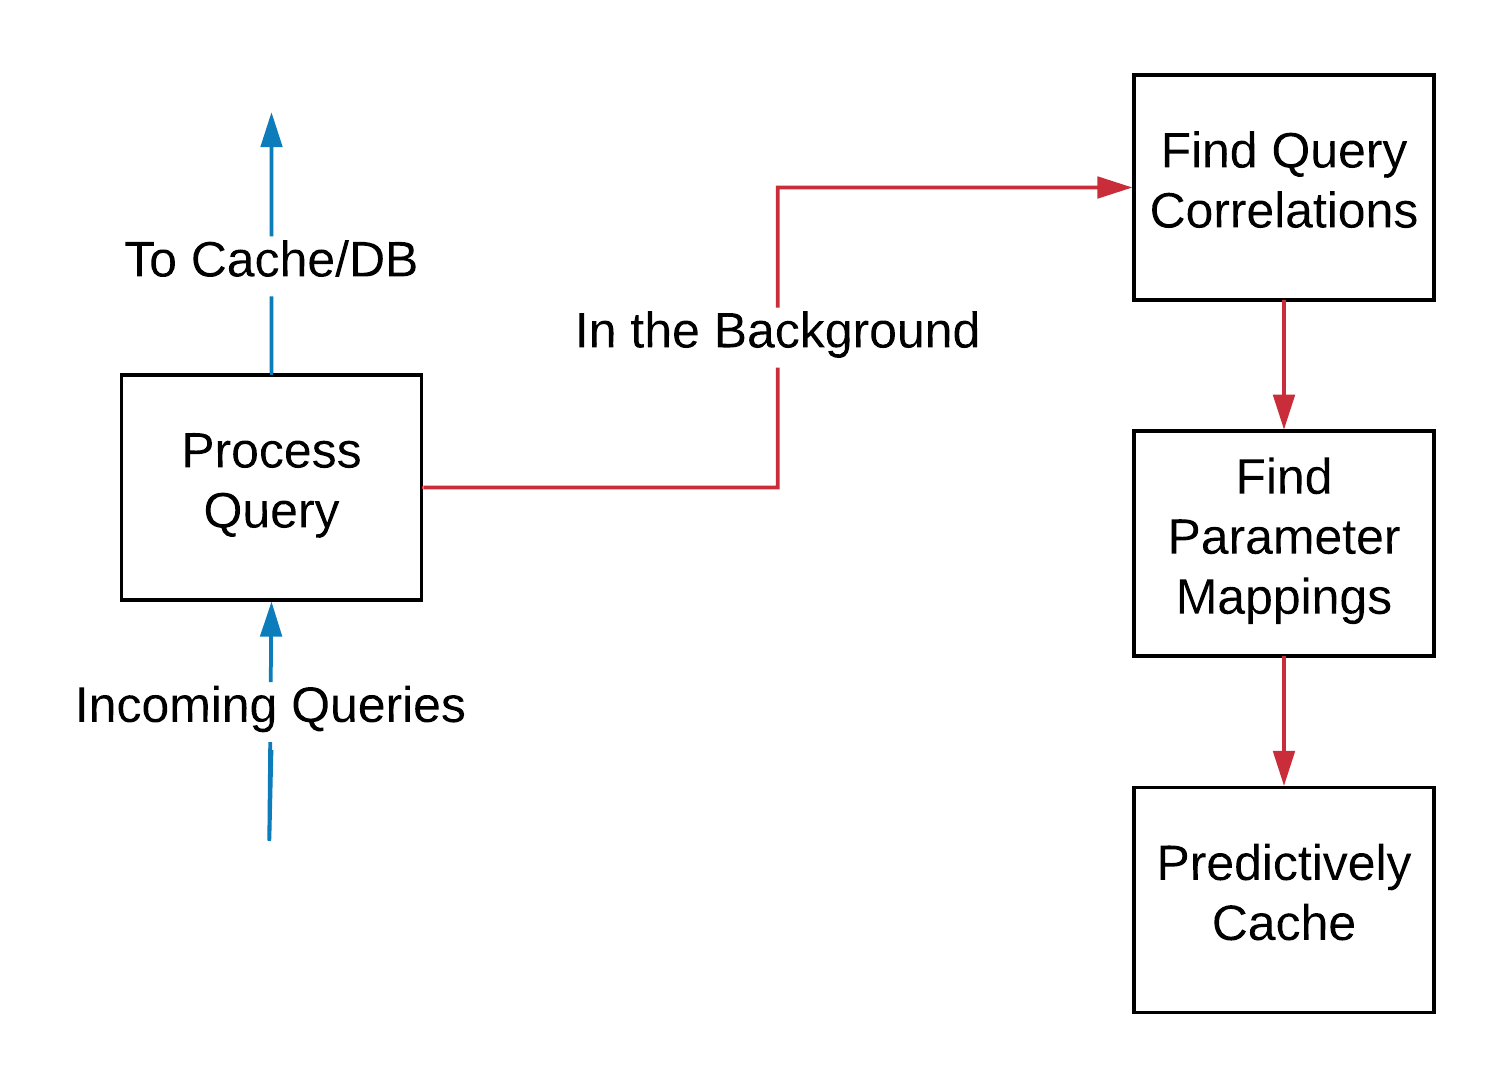
\includegraphics[scale=0.18]{apollo_overview_simplified}
    \end{figure}
\end{frame}



\begin{frame}[fragile]{A Query Submission}
    \begin{center}
SELECT \cfbox{red}{C\_ID} FROM CUSTOMER WHERE
C\_UNAME = 'Alice' and C\_PASSWD = 'pass'

SELECT MAX(O\_ID) FROM ORDERS WHERE
O\_C\_ID = \cfbox{red}{3}
    \end{center}
\end{frame}

\begin{frame}[fragile]{Query Templates}
    Two query instances, $Q_1$, $Q_2$ share the same \alert{query template} if they have the same
    query text modulo \emph{parameterizable constants}.
\end{frame}

\begin{frame}[fragile]{Abstracting Query Instances to Query Templates}
    \begin{center}
SELECT \cfbox{red}{C\_ID} FROM CUSTOMER WHERE
C\_UNAME = \textbf{?} and C\_PASSWD = \textbf{?}

SELECT MAX(O\_ID) FROM ORDERS WHERE
O\_C\_ID = \cfbox{red}{\textbf{?}}
    \end{center}
\end{frame}


\begin{frame}[fragile]{Client Query Streams}
    \begin{figure}
        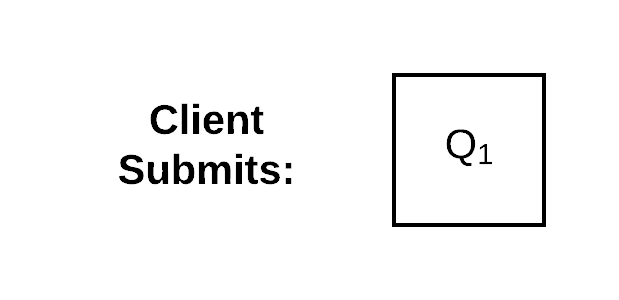
\includegraphics[scale=0.2]{apollo_client_query_stream_0}
    \end{figure}
\end{frame}

\begin{frame}[fragile]{Client Query Streams}
    \begin{figure}
        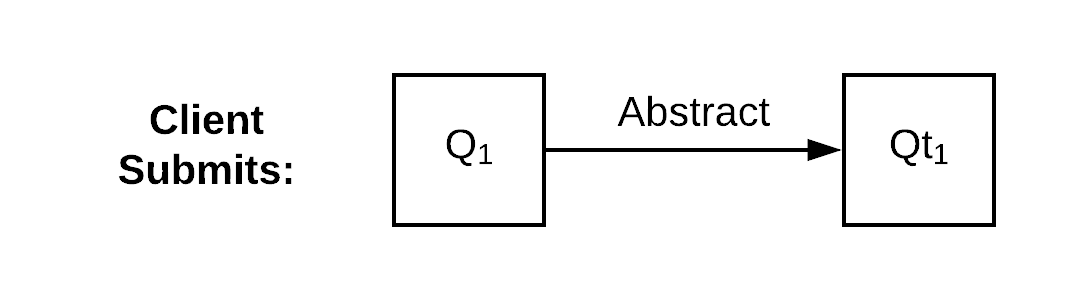
\includegraphics[scale=0.2]{apollo_client_query_stream_0_2}
    \end{figure}

\end{frame}

\begin{frame}[fragile]{Client Query Streams}
    \begin{figure}
        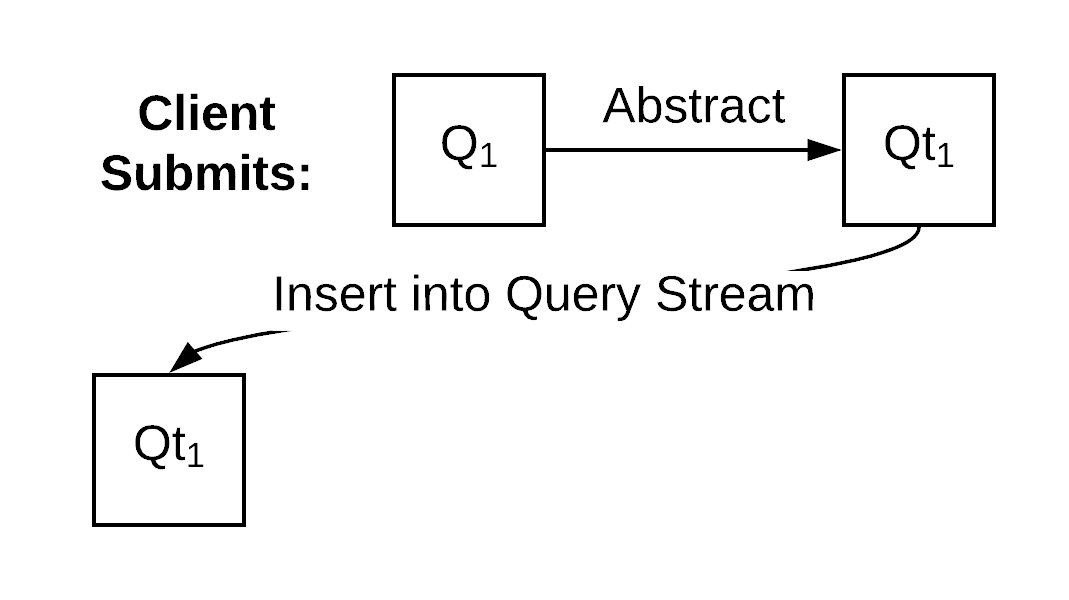
\includegraphics[scale=0.2]{apollo_client_query_stream_0_3}
    \end{figure}
\end{frame}

\begin{frame}[fragile]{Client Query Streams}
    \begin{figure}
        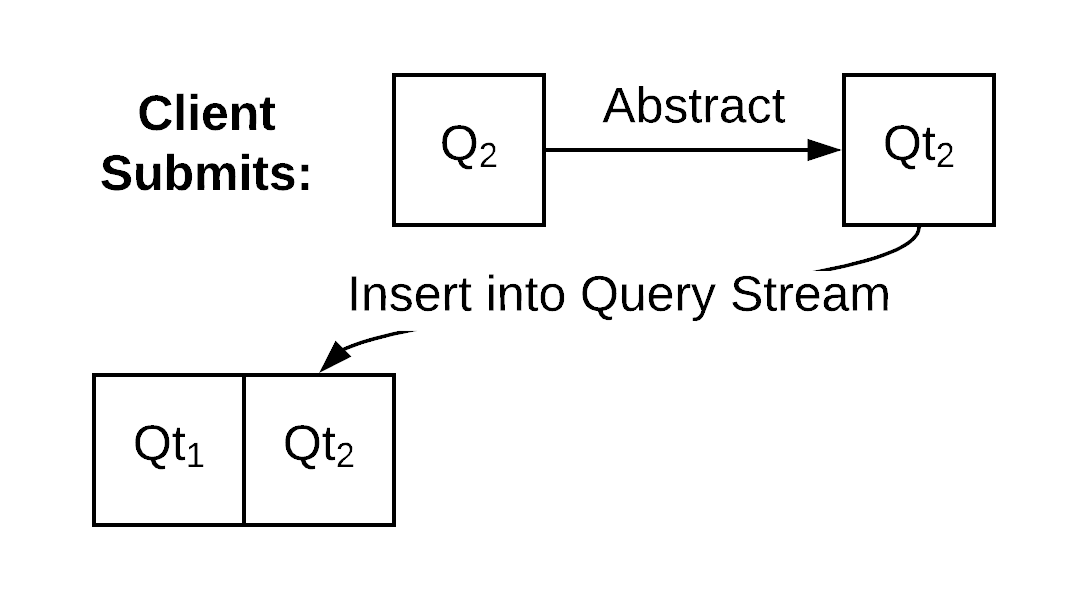
\includegraphics[scale=0.2]{apollo_client_query_stream_0_4}
    \end{figure}
\end{frame}

\begin{frame}[fragile]{Client Query Streams}
    \begin{figure}
        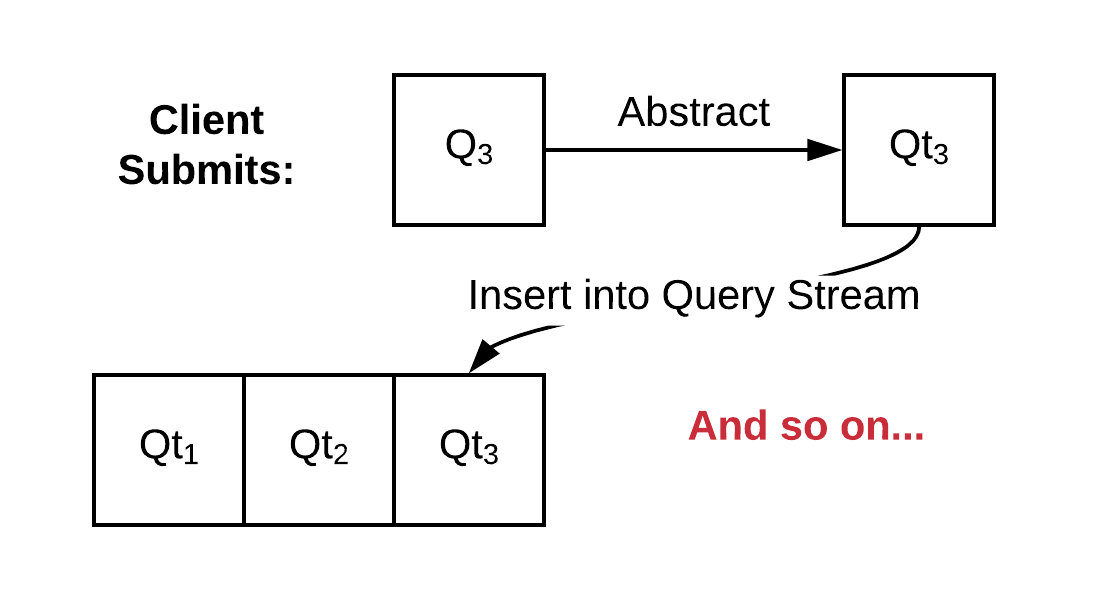
\includegraphics[scale=0.2]{apollo_client_query_stream_0_5}
    \end{figure}
\end{frame}

\begin{frame}[fragile]{Client Query Streams}
    \begin{figure}
        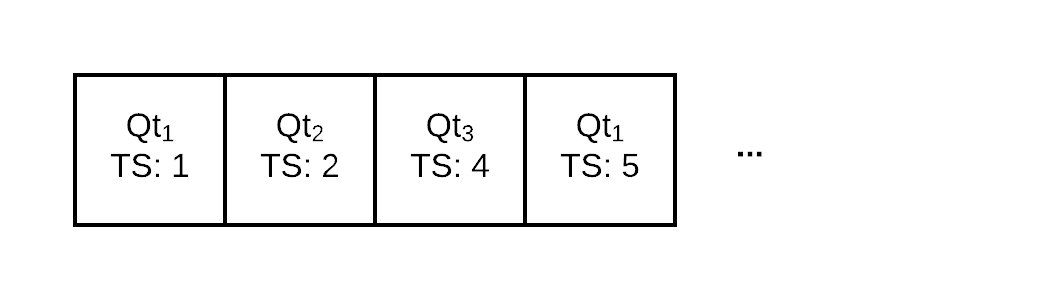
\includegraphics[scale=0.2]{apollo_client_query_stream}
    \end{figure}
\end{frame}

\begin{frame}[fragile]{Client Query Streams}
    \begin{figure}
        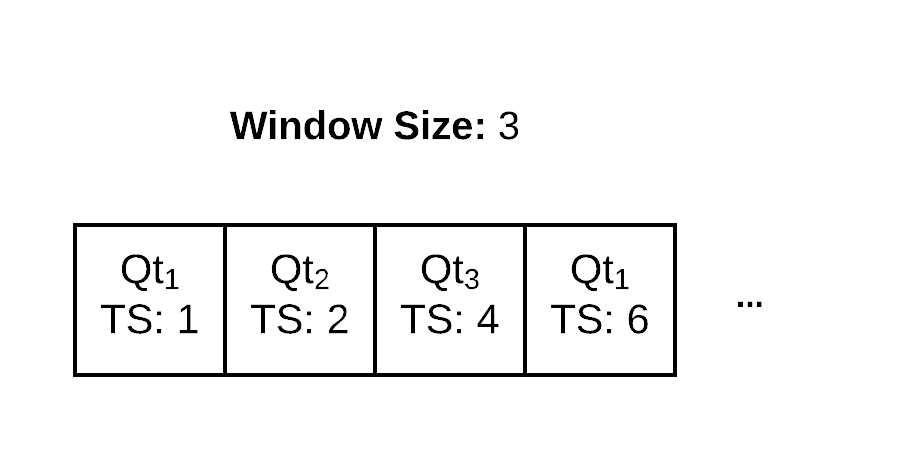
\includegraphics[scale=0.2]{apollo_client_query_stream_2}
    \end{figure}
\end{frame}

\begin{comment}
\begin{frame}[fragile]{Client Query Streams}
    \begin{figure}
        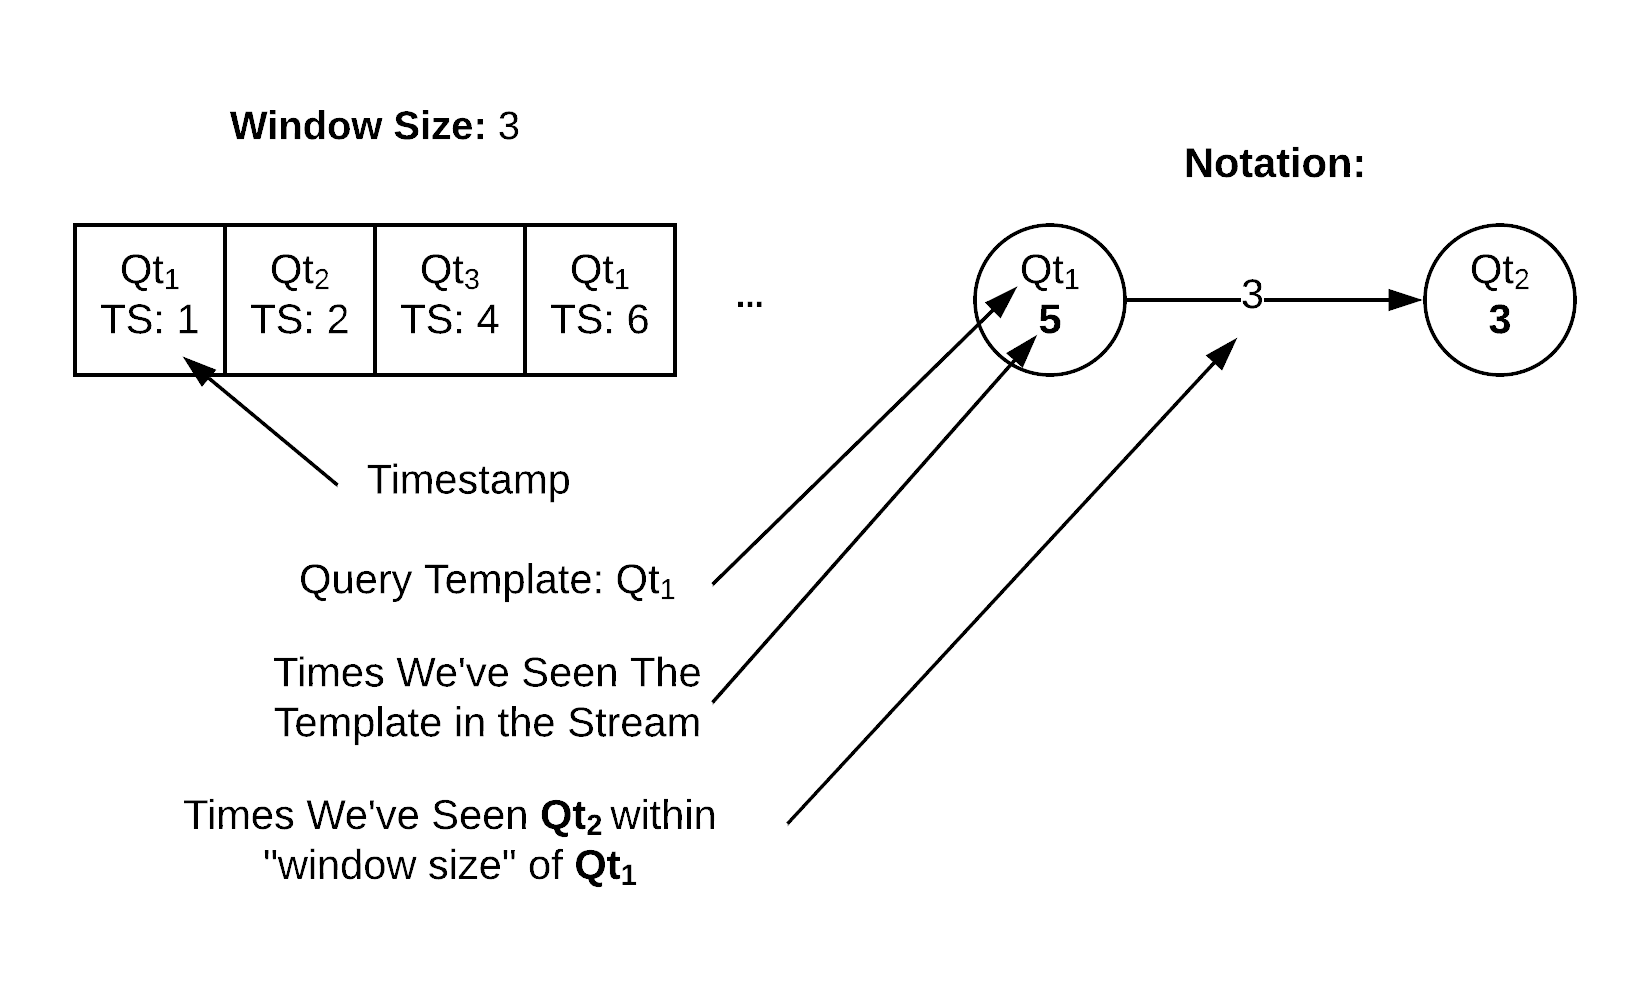
\includegraphics[scale=0.2]{apollo_client_query_stream_2_1}
    \end{figure}
\end{frame}
\end{comment}

\begin{frame}[fragile]{Client Query Streams}
    \begin{figure}
        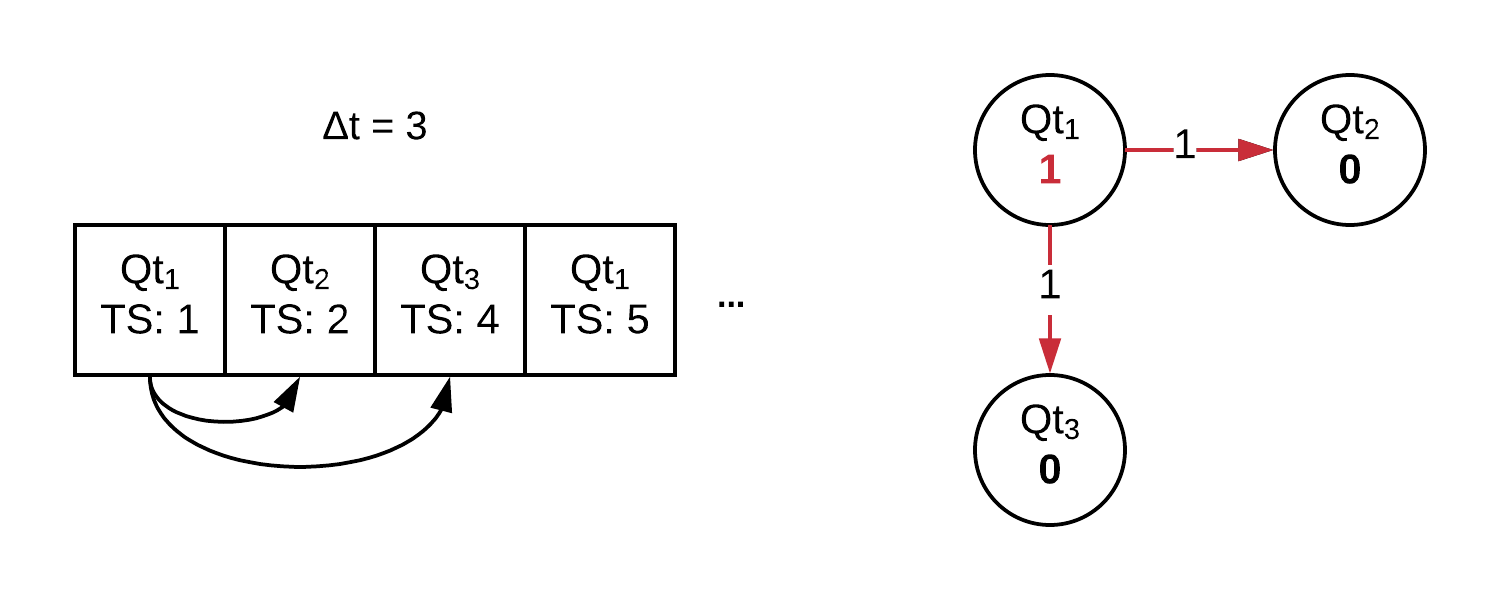
\includegraphics[scale=0.2]{apollo_client_query_stream_3}
    \end{figure}
\end{frame}

\begin{frame}[fragile]{Client Query Streams}
    \begin{figure}
        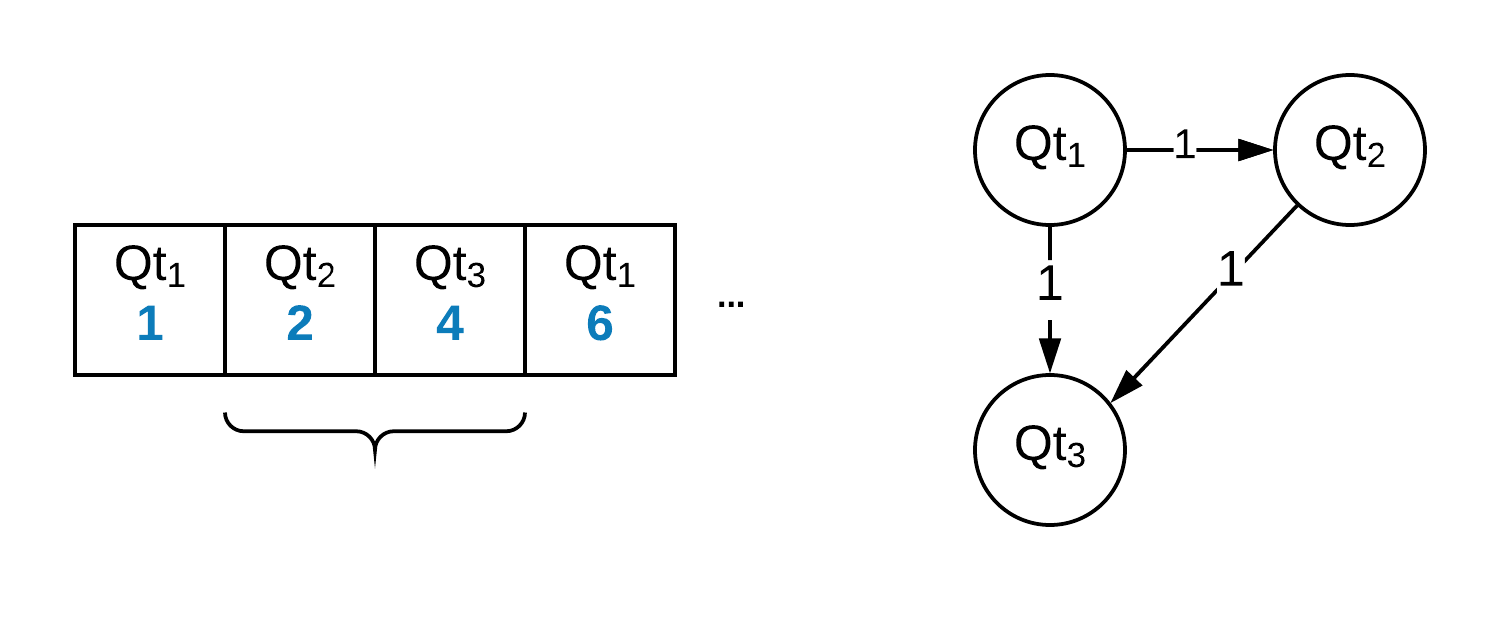
\includegraphics[scale=0.2]{apollo_client_query_stream_4}
    \end{figure}
\end{frame}

\begin{frame}[fragile]{Client Query Streams}
    \begin{figure}
        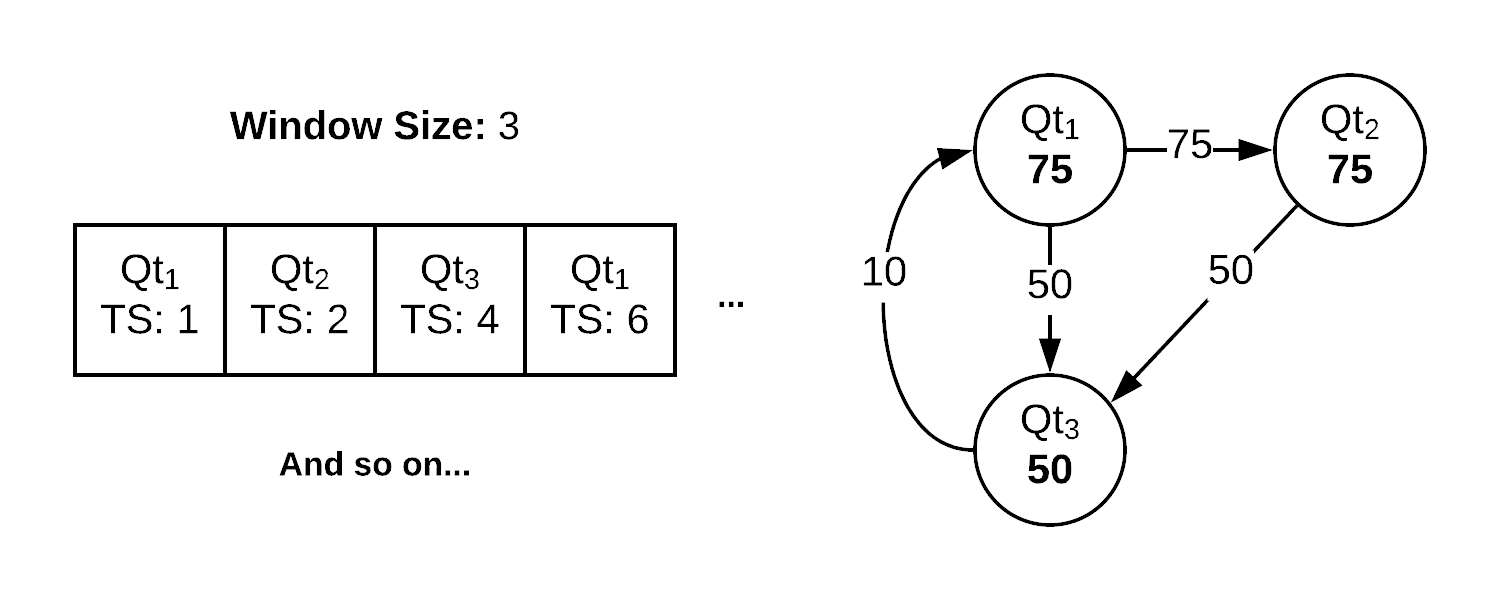
\includegraphics[scale=0.2]{apollo_client_query_stream_5}
    \end{figure}
\end{frame}

\begin{frame}[fragile]{Query Transition Graph}
    \begin{figure}
        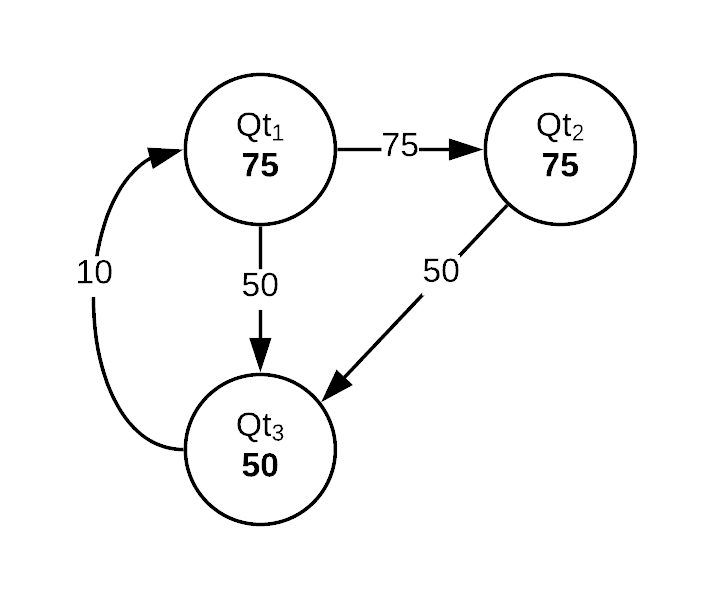
\includegraphics[scale=0.2]{apollo_transition_graph}
    \end{figure}
    \visible<2->{
        Probability of seeing $Qt_{2}$ within sliding window after we've seen $Qt_{1}$:\\
        $P(Qt_{2}|Qt_{1};T\leq\Delta t) = \frac{\textrm{times } Qt_{2} \textrm{ executed within window of } Qt_{1}}{\textrm{times } Qt_{1} \textrm{ executed}} =\frac{75}{75} = 1$\\
    }
    \visible<3->{
        $P(Qt_{1}|Qt_{3};T\leq\Delta t) = \frac{10}{50} = \frac{1}{5}$
    }
\end{frame}

\begin{comment}

\begin{frame}[fragile]{Query Transition Graph}
    The query transition graphs tells us:
    \begin{itemize}
        \item{How often a query template is executed}
        \visible<2->{
        \item{Which query templates are \alert{correlated} with each other. If correlation is sufficiently high ($>$ correlation threshold), then we
        monitor input and output sets for the queries.}
        }
    \end{itemize}
    \visible<3->{
        { \color{red} Need parameter mappings for predictive caching!}
    }
\end{frame}

\end{comment}

\begin{frame}[fragile]{Client Query Streams}
    \begin{figure}
        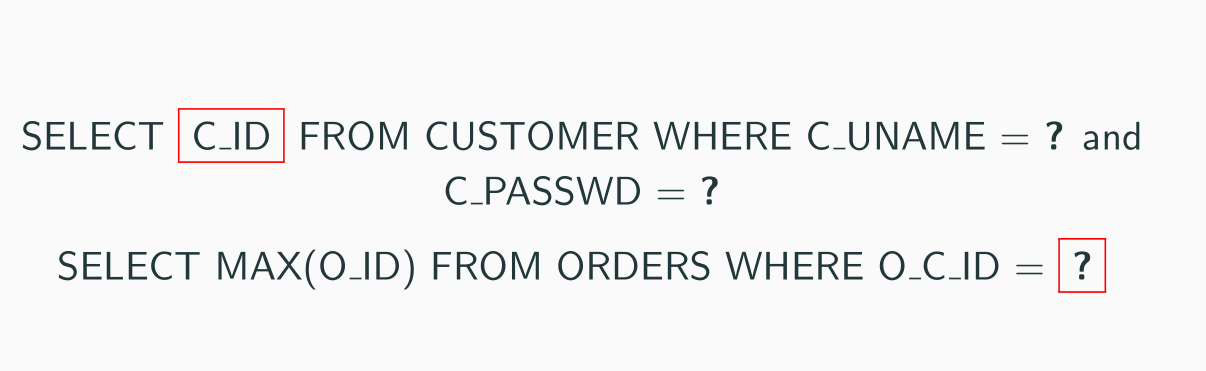
\includegraphics[scale=0.25]{apollo_parameter_mappings}
    \end{figure}
\end{frame}

\begin{frame}[fragile]{Client Query Streams}
    \begin{figure}
        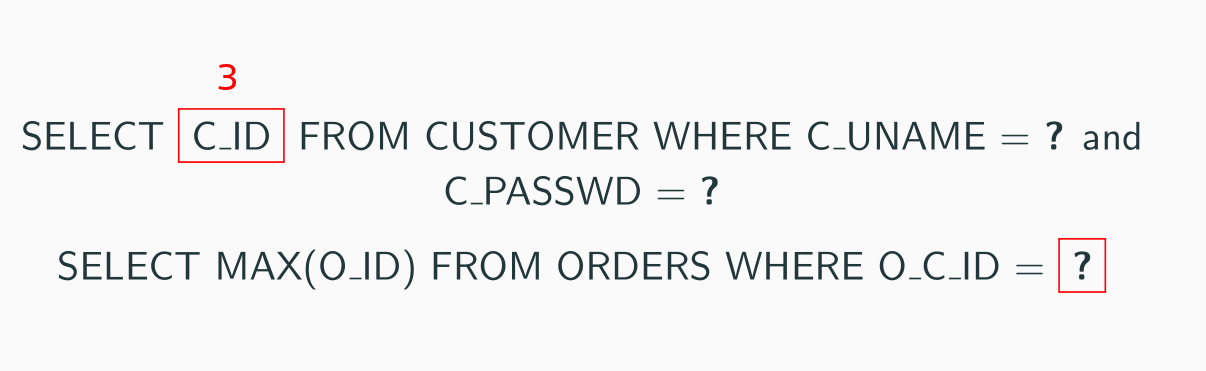
\includegraphics[scale=0.25]{apollo_parameter_mappings_2}
    \end{figure}
\end{frame}

\begin{frame}[fragile]{Client Query Streams}
    \begin{figure}
        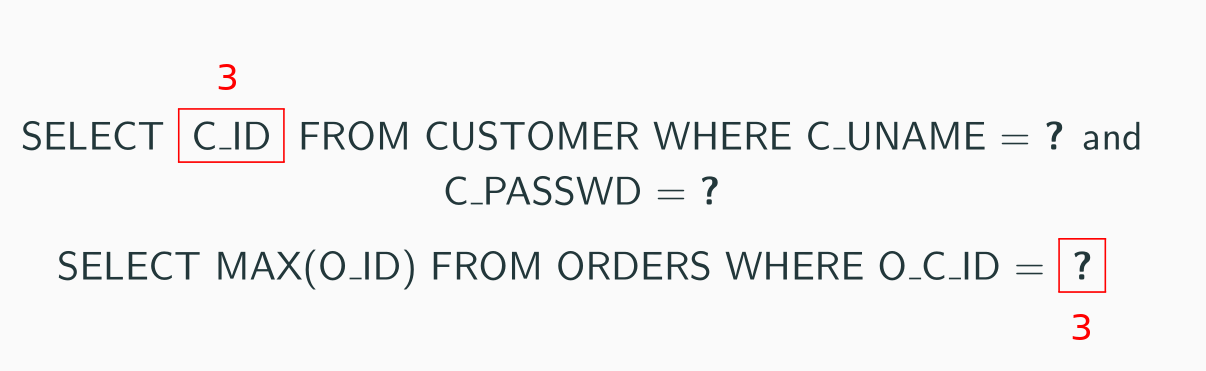
\includegraphics[scale=0.25]{apollo_parameter_mappings_3}
    \end{figure}
\end{frame}

\begin{frame}[fragile]{Client Query Streams}
    \begin{figure}
        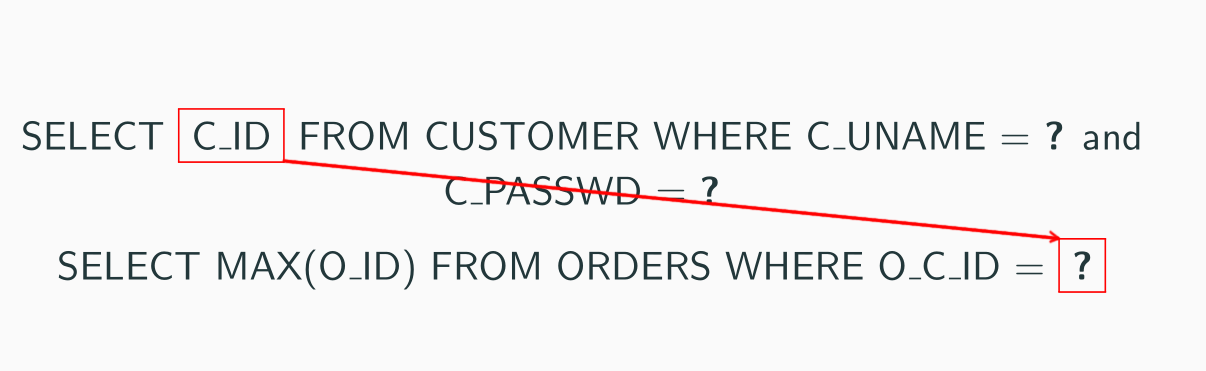
\includegraphics[scale=0.25]{apollo_parameter_mappings_4}
    \end{figure}
\end{frame}

\begin{frame}[fragile]{Dependency Graph}
    \begin{figure}
        \hspace*{-1cm}
        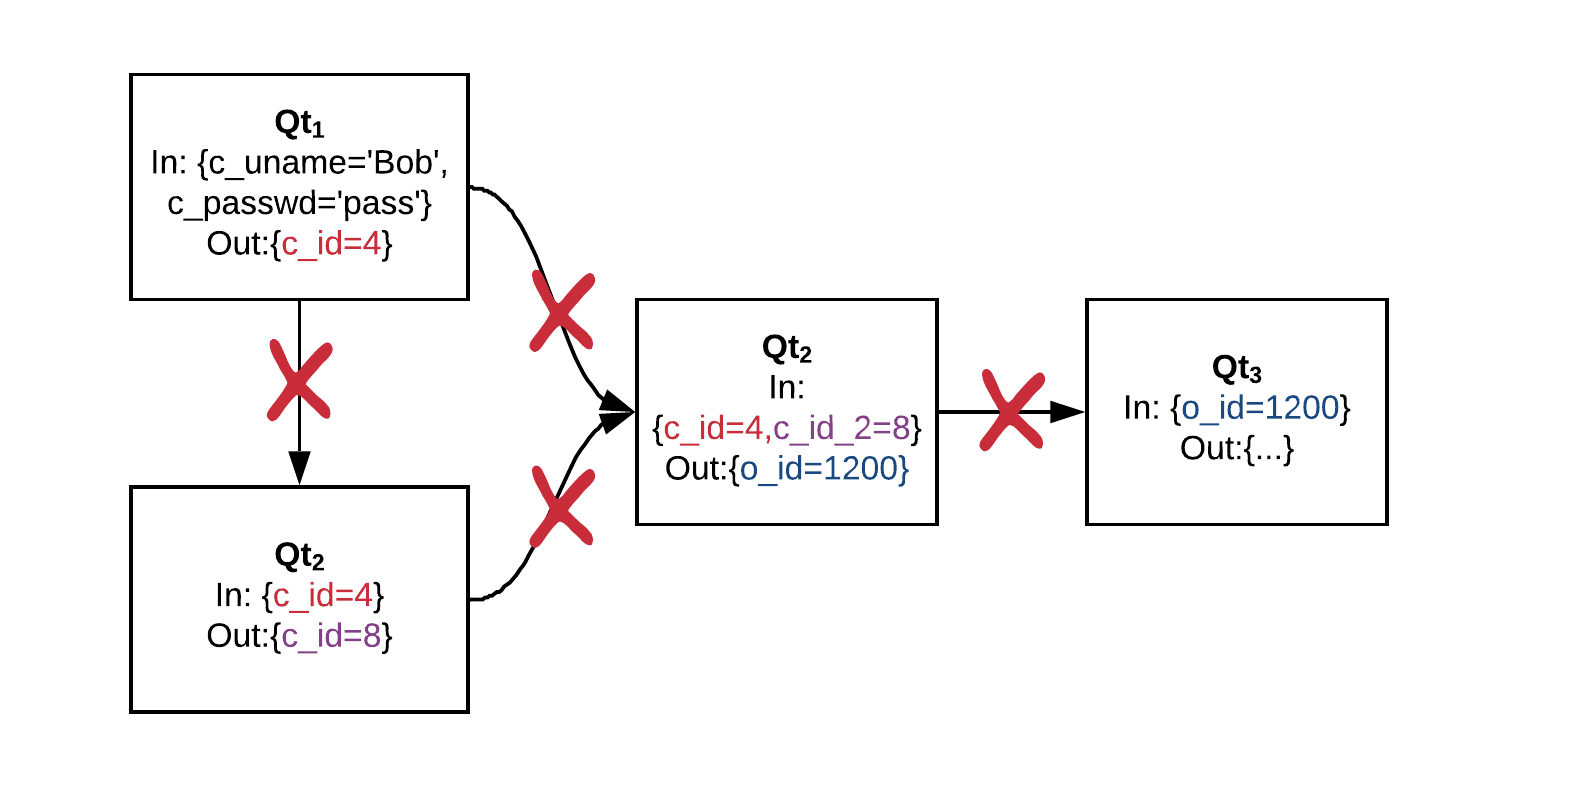
\includegraphics[scale=0.22]{apollo_cpr}
    \end{figure}
\end{frame}

\begin{frame}[fragile]{Core Prediction Routine}
    \begin{figure}
        \hspace*{-1cm}
        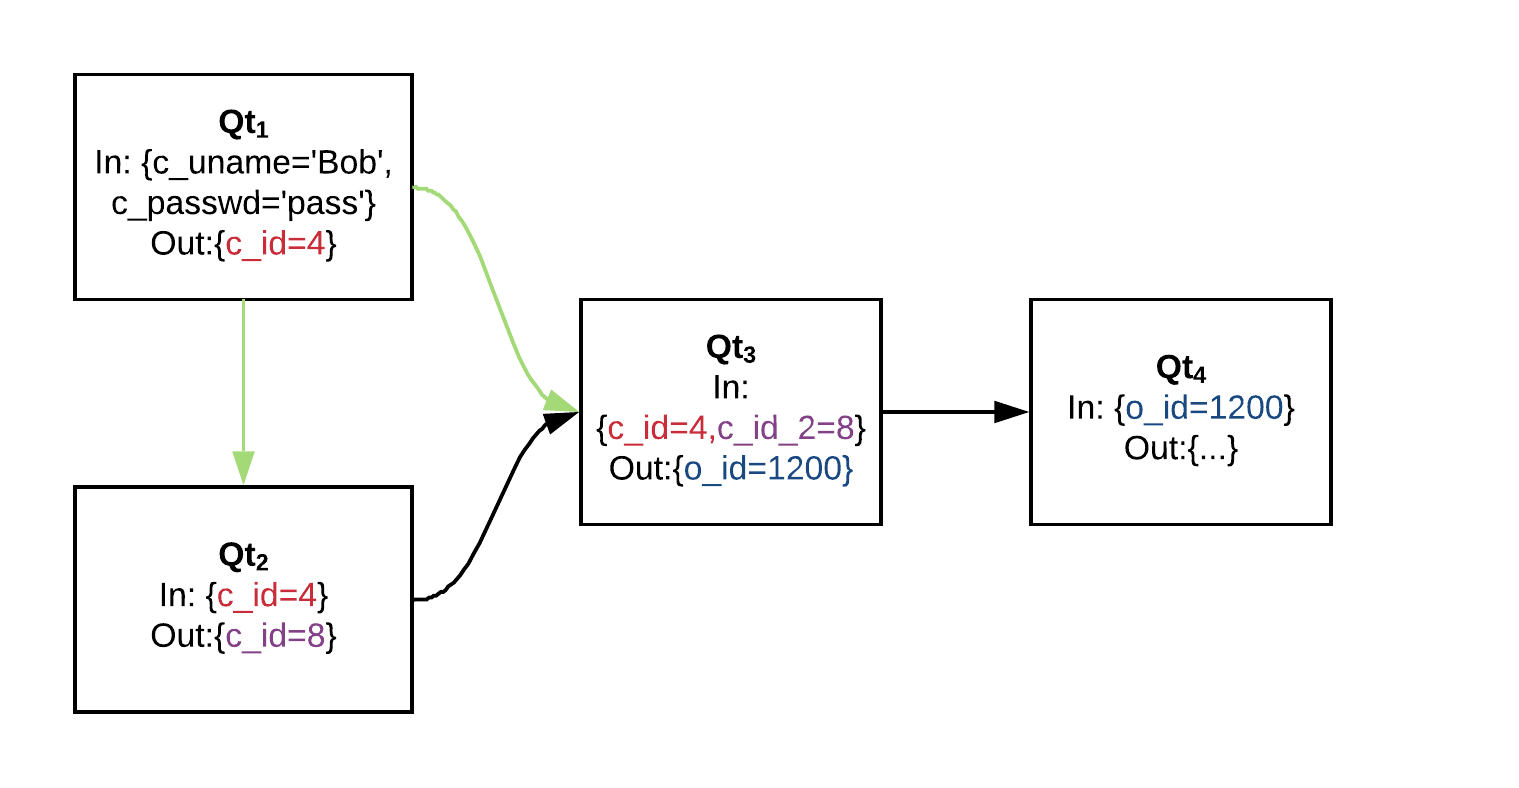
\includegraphics[scale=0.22]{apollo_cpr_2}
    \end{figure}
\end{frame}

\begin{frame}[fragile]{Core Prediction Routine}
    \begin{figure}
        \hspace*{-1cm}
        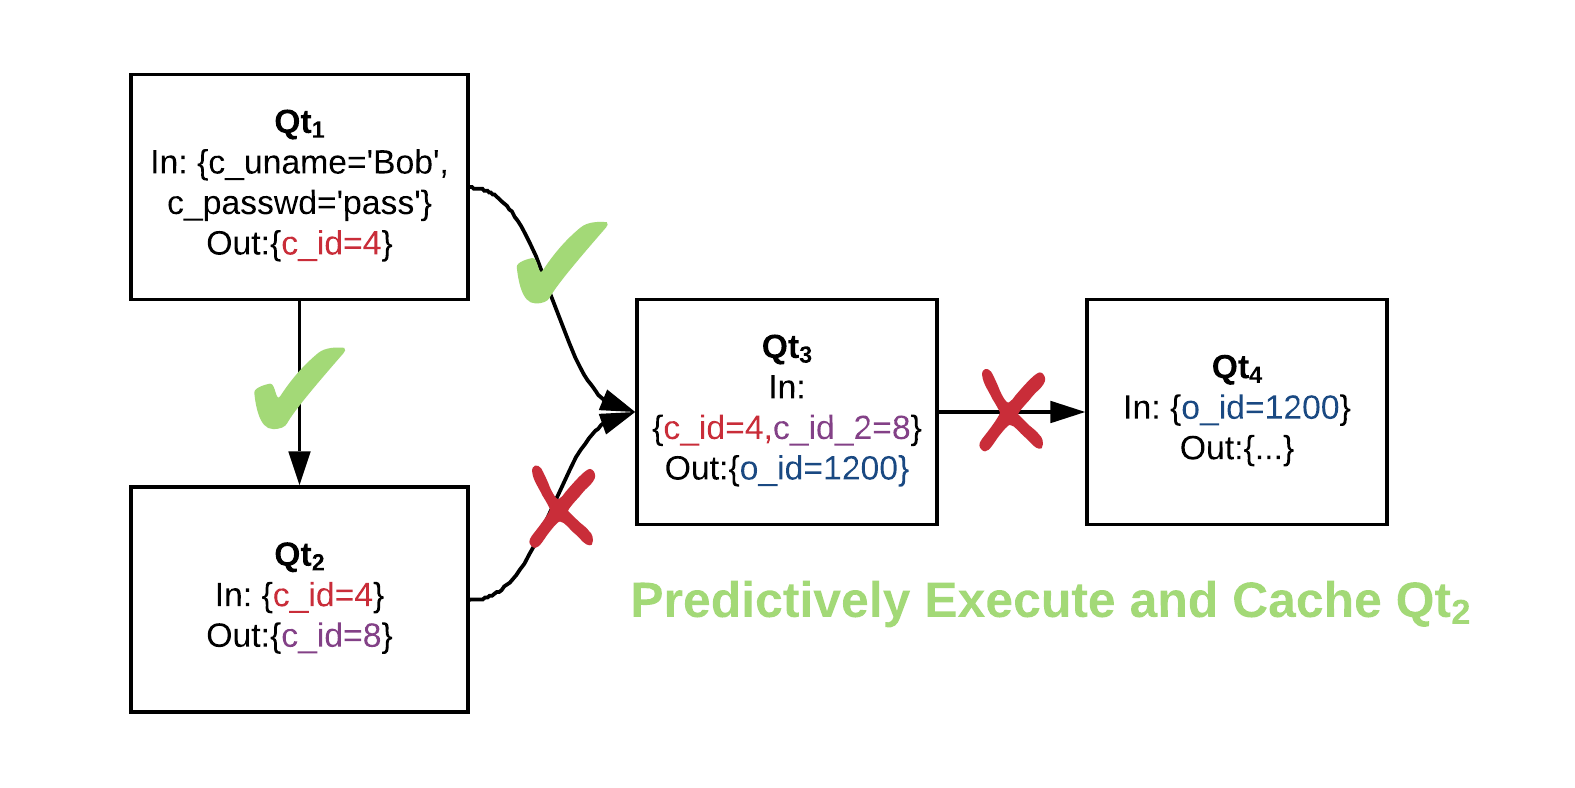
\includegraphics[scale=0.22]{apollo_cpr_3}
    \end{figure}
\end{frame}

\begin{frame}[fragile]{Core Prediction Routine}
    \begin{figure}
        \hspace*{-1cm}
        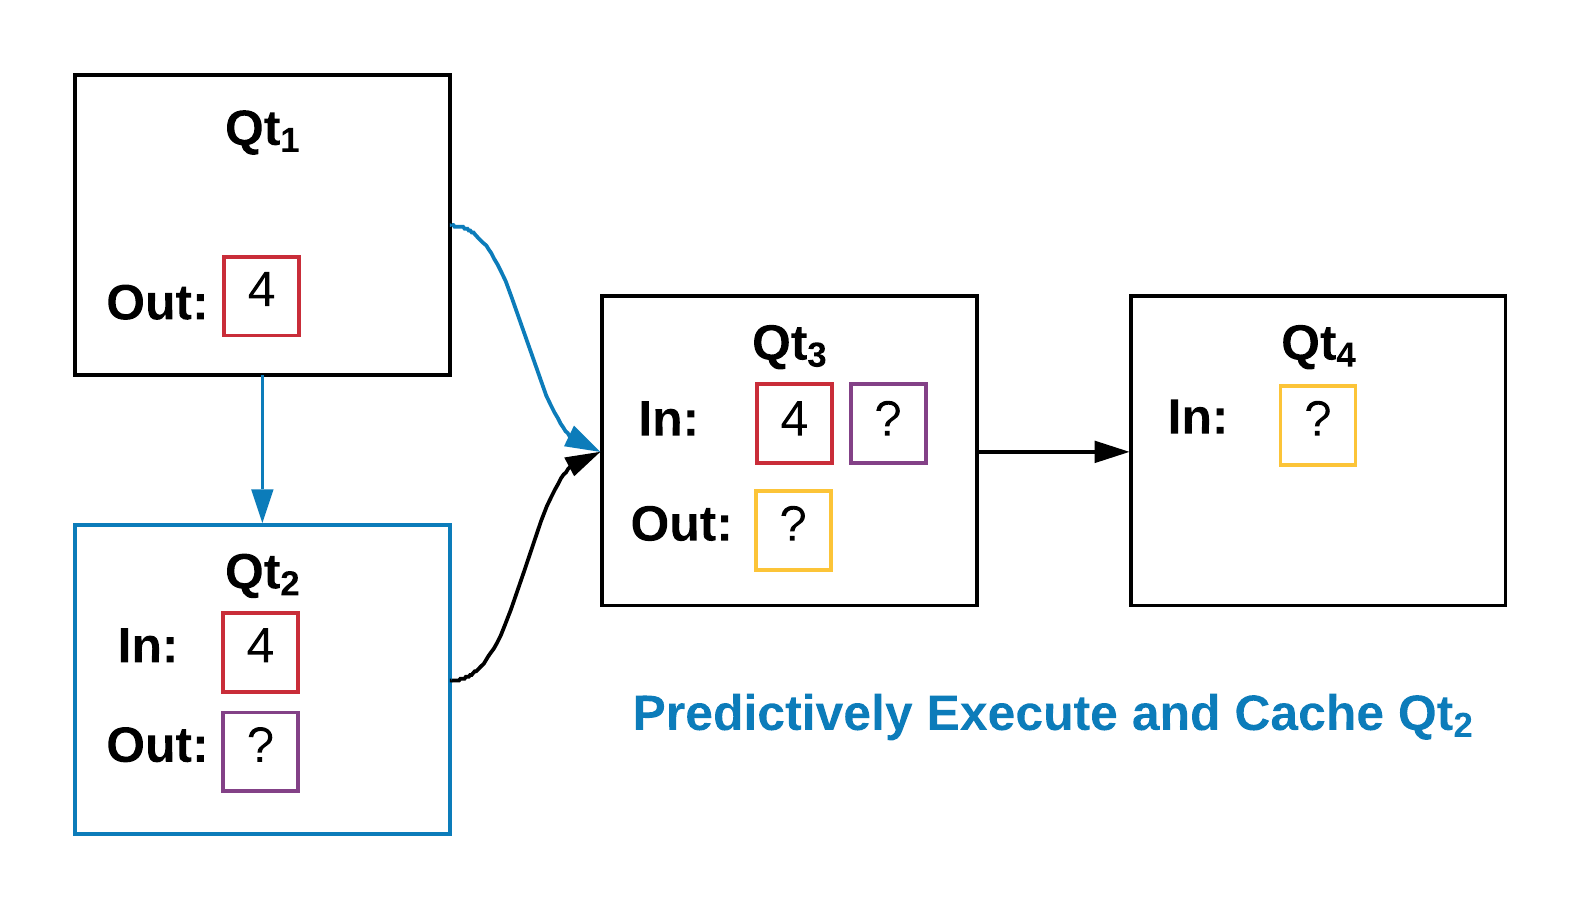
\includegraphics[scale=0.22]{apollo_cpr_4}
    \end{figure}
\end{frame}

\begin{frame}[fragile]{Core Prediction Routine}
    \begin{figure}
        \hspace*{-1cm}
        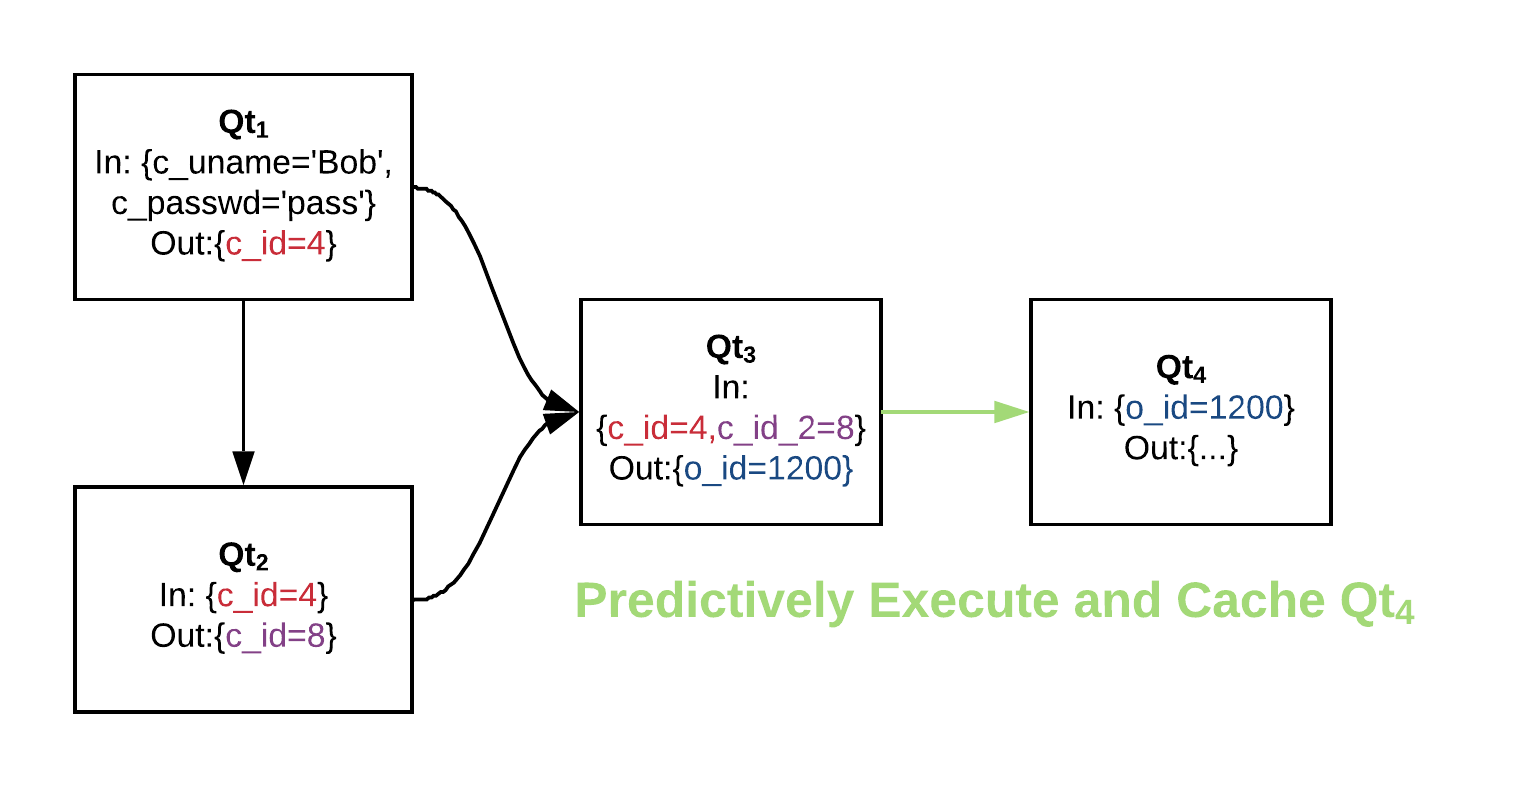
\includegraphics[scale=0.22]{apollo_cpr_5}
    \end{figure}
\end{frame}

\begin{frame}[fragile]{Core Prediction Routine}
    \begin{figure}
        \hspace*{-1cm}
        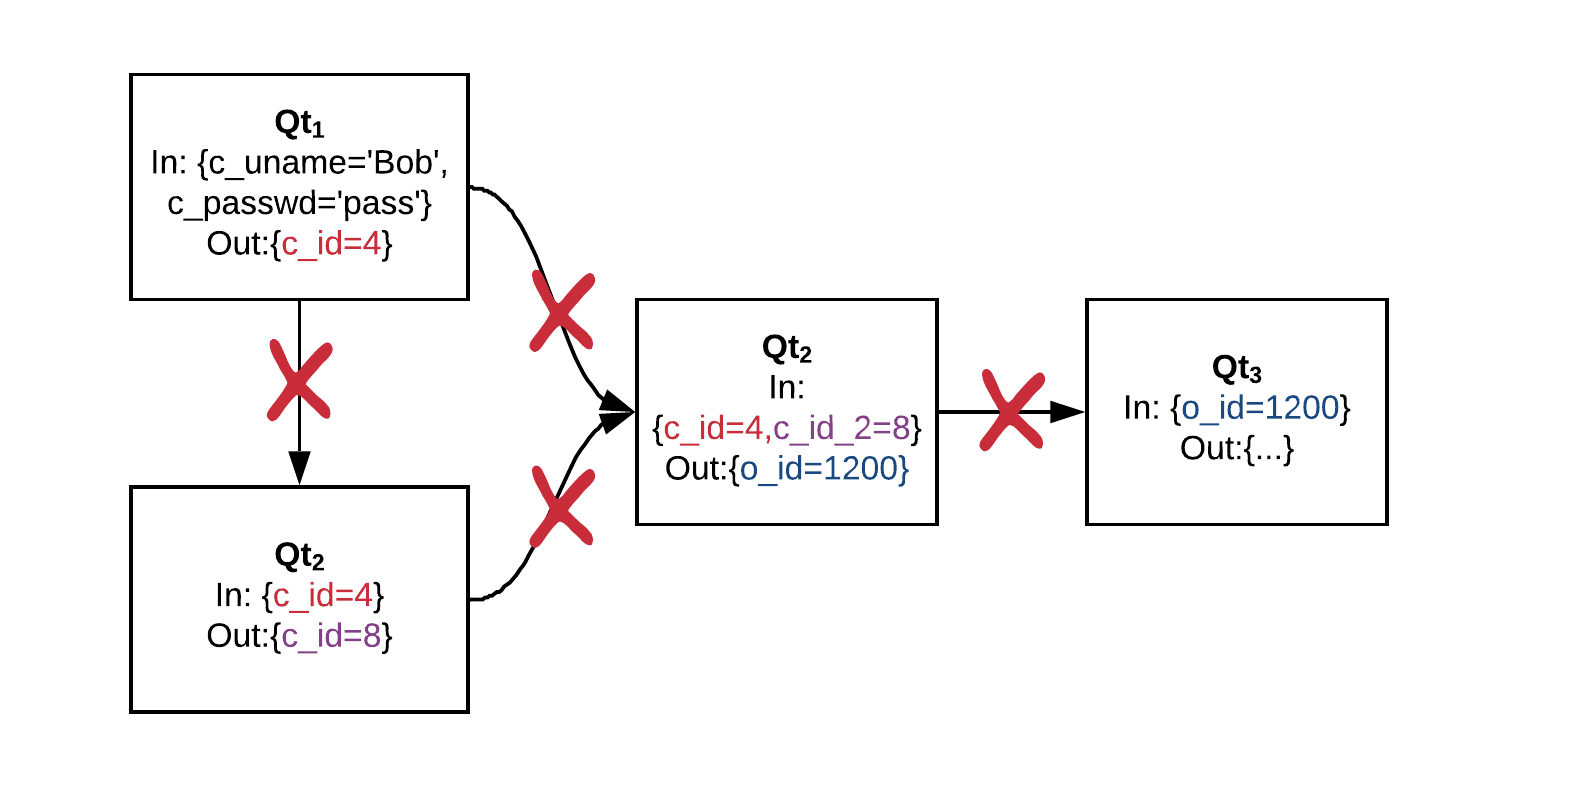
\includegraphics[scale=0.22]{apollo_cpr}
    \end{figure}
\end{frame}

\section{Invalidation}

\begin{frame}[fragile]{Client-Centric Caching}
    \begin{figure}
        \hspace*{-1cm}
        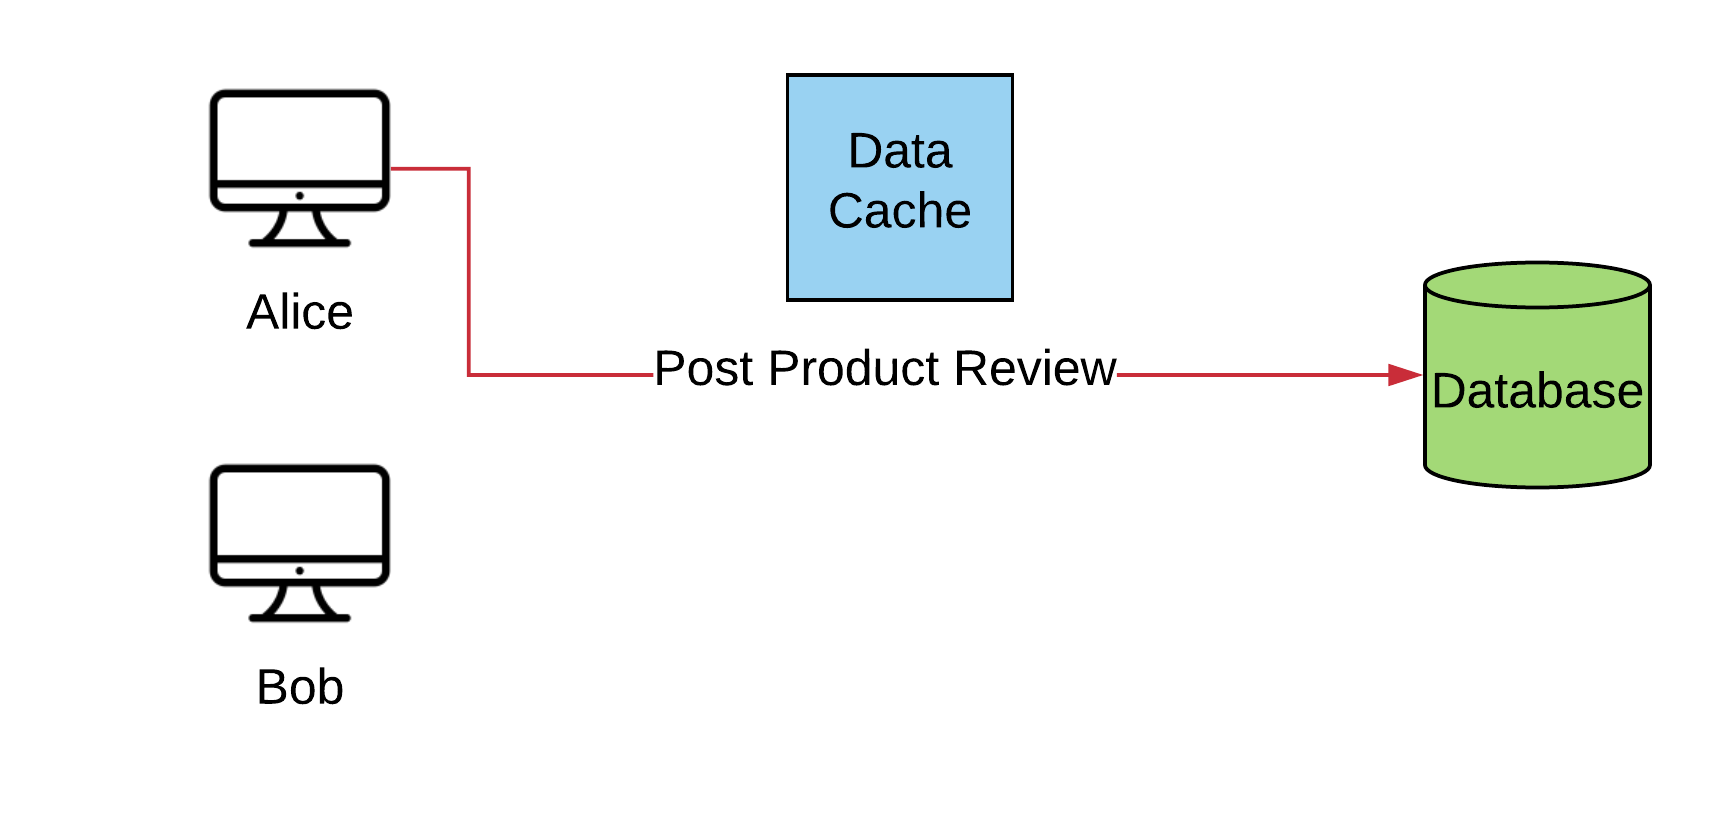
\includegraphics[scale=0.19]{apollo_client_sessions_simplified}
    \end{figure}
    \bigskip
    \medskip
    \smallskip
    \bigskip
    \medskip
    \smallskip
\end{frame}

\begin{frame}[fragile]{Client-Centric Caching}
    \begin{figure}
        \hspace*{-1cm}
        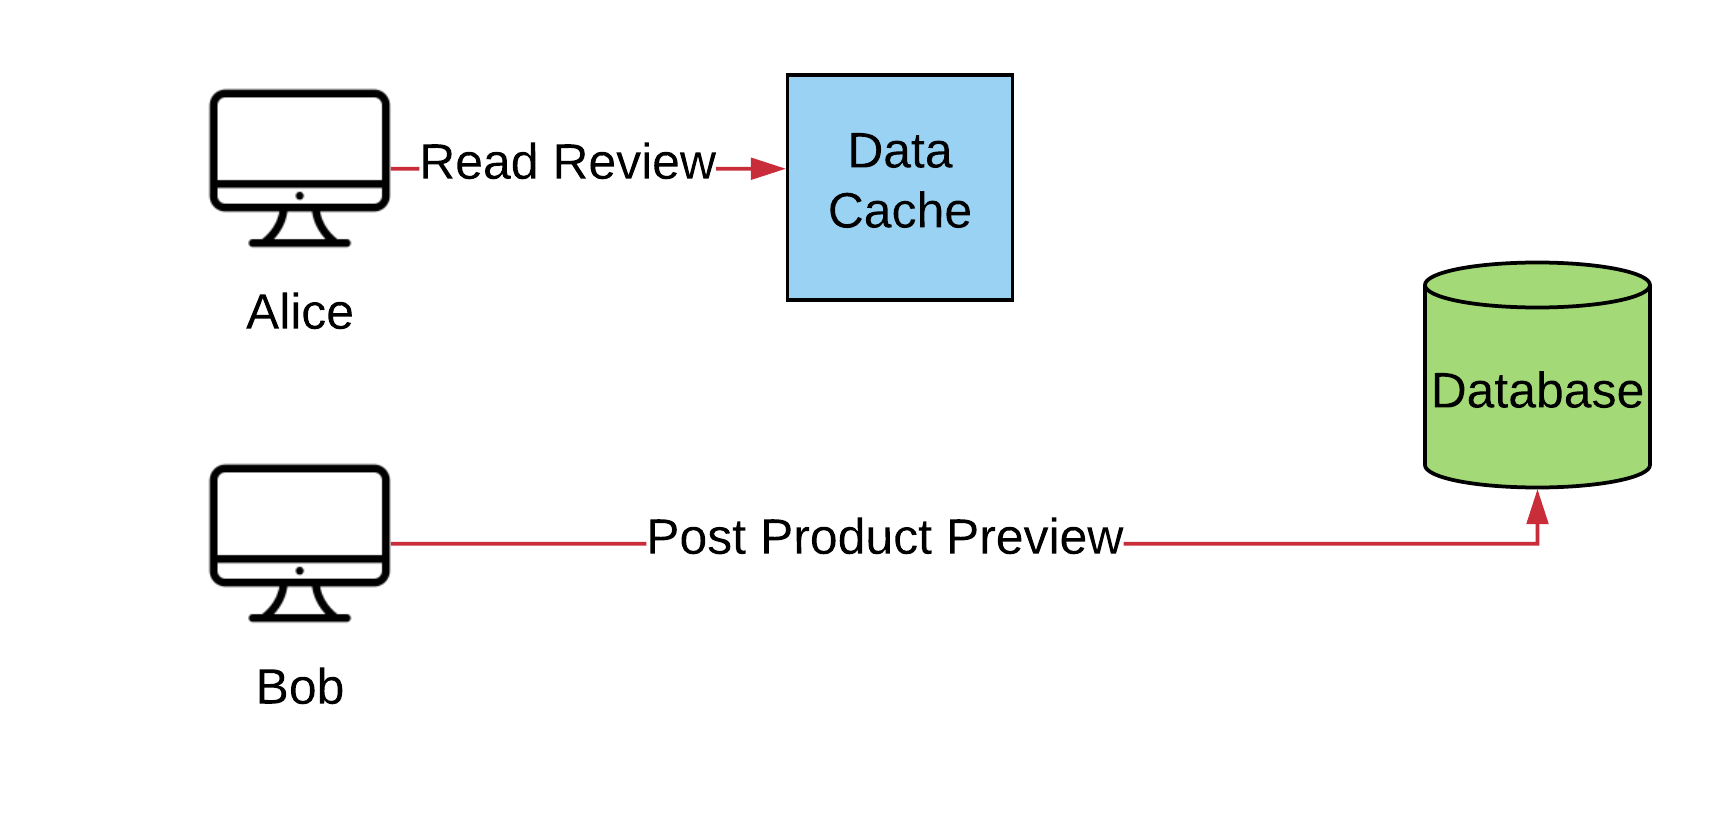
\includegraphics[scale=0.19]{apollo_client_sessions_simplified_2}
    \end{figure}
    \visible<2->{
    Alice should \alert{see her own order}, but does not care about Bob's!
    }
    \begin{itemize}
    \visible<3->{
        \item{Improves cache performance, \alert{client-centric} model}
        \item{Support for reading latest data if needed}
    }
    \end{itemize}
\end{frame}

\begin{frame}{Benefits of Client-Centric Caching}
    \begin{figure}
        \center
        \hspace*{-1.5cm}
        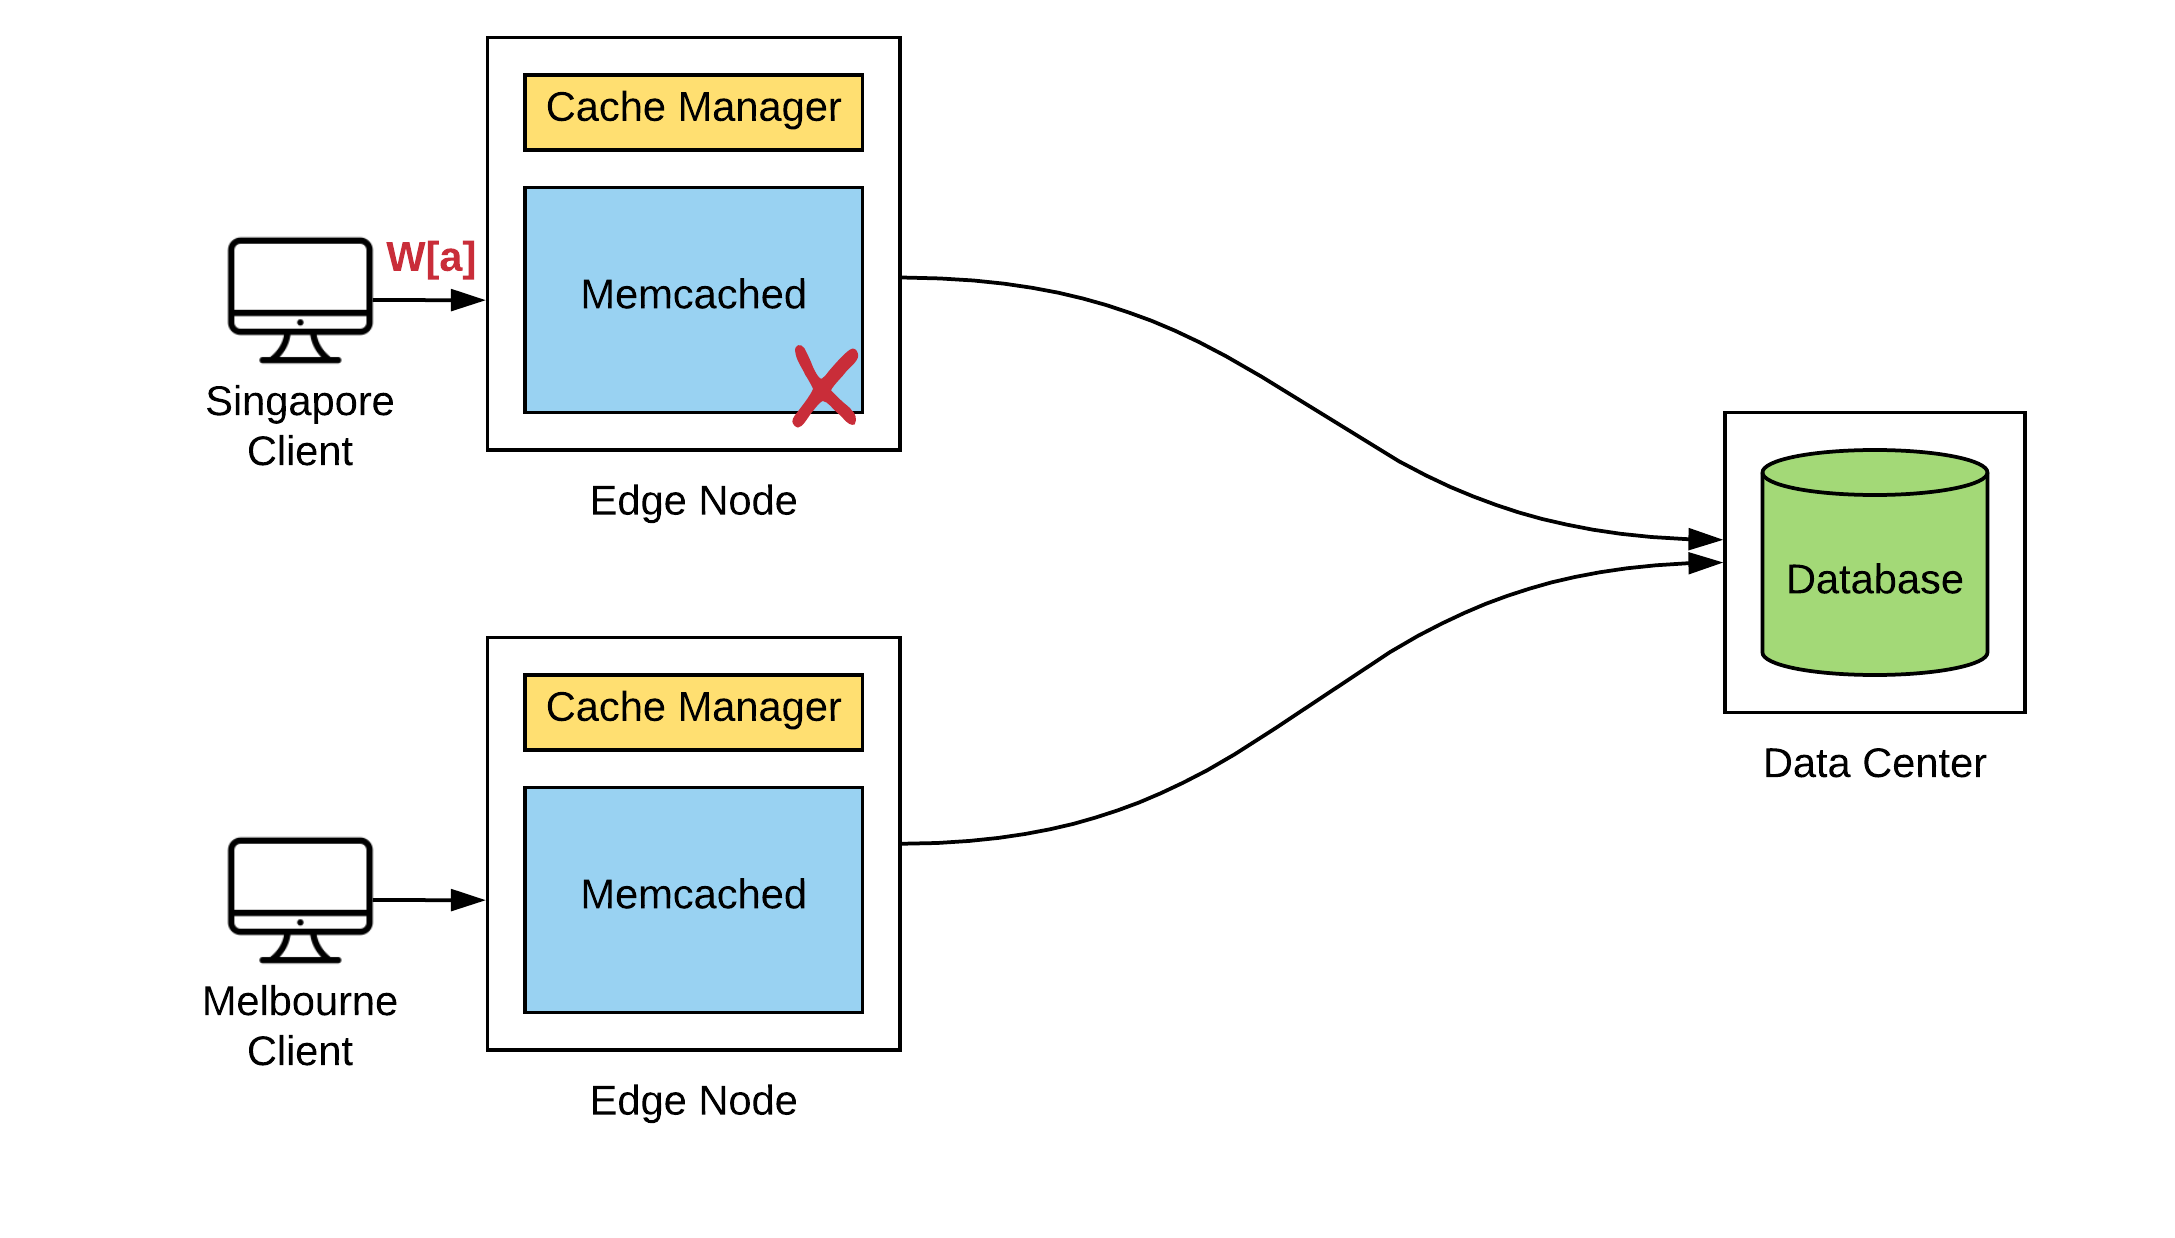
\includegraphics[scale=0.17]{apollo_ec_upd}
    \end{figure}
\end{frame}

\begin{frame}[fragile]{Benefits of Client-Centric Caching}
    \begin{itemize}
        \item{Can predict whether a prefetched query result will be used before invalidation!}
        \item{Reloading queries upon invalidation}
    \end{itemize}
   \alert{See paper for details!}
\end{frame}

\section{Experiments}

\begin{frame}[fragile]{Experiment Configuration}
    \begin{figure}
        \center
        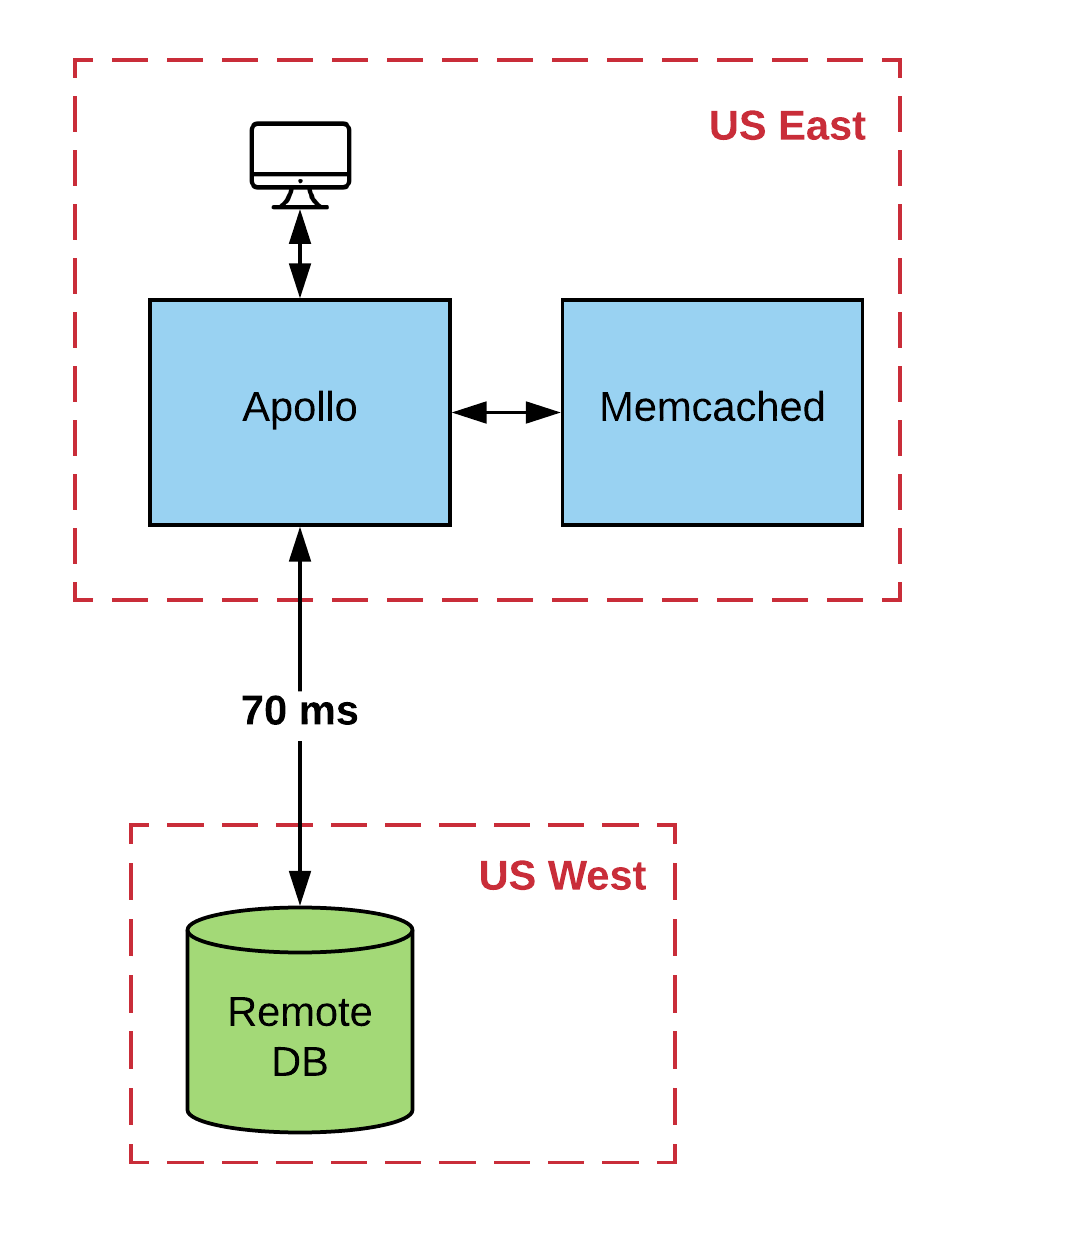
\includegraphics[scale=0.17]{apollo_exp_config}
    \end{figure}
\end{frame}

\begin{frame}[fragile]{Experiment Configuration}
    Three configurations:
    \begin{itemize}
        \item{\alert{Apollo configuration:} as described in prior sections.}
        \item{\alert{Memcached configuration:} LRU cache --- Apollo with predictive features turned off}
        \item{\alert{Fido configuration:} Use Fido predictive engine instead of Apollo's predictive features!}
    \end{itemize}
\end{frame}

\begin{frame}[fragile]{Fido}
    \begin{figure}
        \center
        \includegraphics[scale=0.3]{apollo_fido_pred}
    \end{figure}
\end{frame}

\begin{frame}[fragile]{Fido}
    \begin{figure}
        \center
        \includegraphics[scale=0.3]{apollo_fido_pred_2}
    \end{figure}
\end{frame}

\begin{frame}[fragile]{Fido}
    \begin{itemize}
        \item{\alert{Query instance} based predictions, instead of query templates.}
        \item{Prefix length: 3, Suffix Length: 2}
        \item{Requires offline training (Supplied 40 minutes of data).}
    \end{itemize}
\end{frame}

\begin{frame}[fragile]{TPC-W Results}
    \begin{figure}
        \center
        \includegraphics[scale=0.7]{apollo_tpcw}
    \end{figure}
\end{frame}

\begin{frame}[fragile]{Learning Over Time}
    \begin{figure}
        \center
        \includegraphics[scale=0.7]{apollo_30_intervals}
    \end{figure}
\end{frame}

\begin{frame}[fragile]{Workload Change}
    \begin{figure}
        \center
        \includegraphics[scale=0.11]{apollo_wl_change}
    \end{figure}
\end{frame}

\begin{frame}[fragile]{Predictive Caching \emph{Works}}
Broad conclusions
\begin{centering}
Questions?
\end{centering}
\end{frame}

\begin{frame}[fragile]{Multiple Apollo Instances}
    \begin{figure}
        \center
        \includegraphics[scale=0.7]{apollo_scalability_curve}
    \end{figure}
\end{frame}

\begin{frame}[fragile]{Parameter Settings (TPC-W)}
\begin{table}
\centering
\begin{tabular}{ll}
Parameter & Setting \\
\toprule
Window Width & 15s \\
Correlation Threshold & 0.99 \\
Reload Threshold & 0 \\
Cache Size & 5\% of DB \\
\bottomrule
\end{tabular}
\end{table}

\end{frame}

\begin{frame}[fragile]{Related Work (Systems)}
\begin{table}
\centering
\begin{tabular}{lll}
\multicolumn{3}{c}{Similarities and Differences Among Related Work} \\
\toprule
System & Similarities & Differences \\
\midrule
\textbf{Scalpel} & \multicolumn{1}{p{5cm}}{\tabitem{Prefetching via templates}} & \tabitem{Offline training}  \\
& & \tabitem{Write Handling} \\
& & \tabitem{Client-side} \\
& & \tabitem{Query Rewriting} \\
\midrule
\textbf{Fido} & \tabitem{Prefetching} & \tabitem{Offline training} \\
& \tabitem{Server-side/middleware} & \tabitem{Query Instances} \\
& & \tabitem{Write Handling} \\
\midrule
\end{tabular}
\end{table}
\end{frame}

\begin{frame}[allowframebreaks]
    \bibliographystyle{abbrv}
    \bibliography{demo}
\end{frame}


\end{document}
